% !TEX root = ../main.tex

\chapter{Preliminares}
\label{chap:preliminares}

\section{Variedades diferenciáveis e Diferenciabilidade}
\label{loc:variedades_diferenciáveis_e_diferenciabilidade}
Começaremos por apresentar alguns conceitos fundamentais da Topologia Diferencial, os quais serão indispensáveis para o texto.

O primeiro deles, que é o principal objeto de estudo da Topologia Diferencial e serve como uma generalização das superfícies contidas em $\mathbb{R}^{3}$, é o conceito de variedade diferenciável. De forma análoga a superfícies, uma variedade diferenciável é um conjunto que se comporta localmente como o espaço euclidiano $\mathbb{R}^{n}$. A definição formal desse conceito é a seguinte:
\begin{definition}
    \label{loc:2.1_:_def_1_:_variedade_diferenciável.definição}
    Uma variedade diferenciável de dimensão $n$ é um conjunto $M$, e uma família $\{ (U_{\alpha}, \mathbf{x}_{\alpha}) \}$, onde os $U_{\alpha}$ são abertos do $\mathbb{R}^{n}$, e $\mathbf{x}_{\alpha}:U_{\alpha}\to M$ são bijeções, satisfazendo:
    \begin{enumerate}
        \item $\cup_{\alpha} \mathbf{x}_{\alpha}(U_{\alpha})=M$
        \item Se $\alpha$ e $\beta$ são índices, tais que $\mathbf{x}_{\alpha}(U_{\alpha})\cap \mathbf{x}_{\beta}(U_{\beta}) = W \neq \emptyset$ e $\mathbf{x}^{-1}_{\alpha}(W)$ e $\mathbf{x}^{-1}_{\beta}(W)$ são abertos do $\mathbb{R}^{n}$, então $\mathbf{x}_{\beta}^{-1} \circ\mathbf{x}_{\alpha}|_{\mathbf{x_{\alpha}^{-1}(W)}}$ é uma função diferenciável.
        \item A família $\{ (U_{\alpha}, \mathbf{x}_{\alpha}) \}$ é maximal relativamente às condições 1) e 2).
    \end{enumerate}

    Uma família $\{ (V_{\alpha}, \mathbf{y}_{\alpha}) \}$ satisfazendo 1) e 2) (não necessariamente maximal) é chamada de estrutura diferencial de $M$. Note aqui que tal família é compatível com a família maximal de $M$, isto é, $\{ (V_{\alpha}, \mathbf{y}_{\alpha}) \} \subset\{ (U_{\alpha}, \mathbf{x}_{\alpha}) \}$.
    \begin{center}

        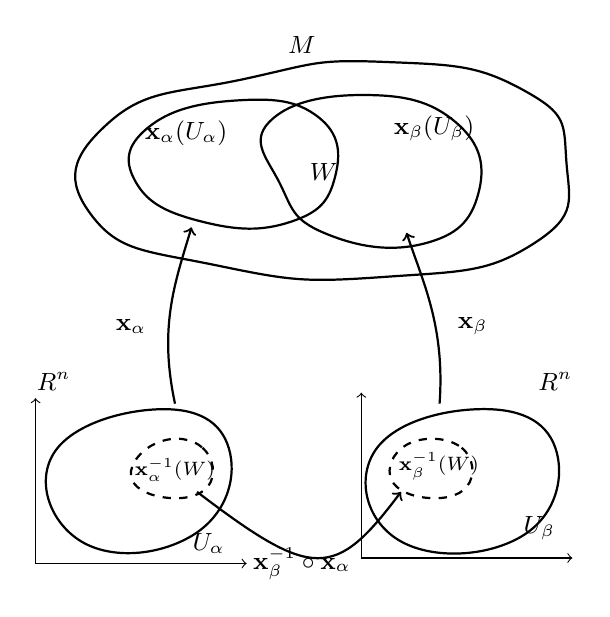
\begin{tikzpicture}[scale=0.7, every node/.style={font=\small}]

            % ---------- Manifold M (top) ----------
            \draw[thick] plot [smooth cycle, tension=0.9] coordinates {
                    (-3.5,5.5) (-1,6.3) (1.5,6.6) (4,6.1) (4.8,4.8)
                    (4.2,3.3) (1.5,2.7) (-1.5,2.9) (-3.8,3.8)
                };
            \node at (0,6.9) {$M$};

            % region x_alpha(U_alpha)
            \draw[thick] plot [smooth cycle, tension=0.8] coordinates {
                    (-2.8,5.4) (-1.2,5.9) (0.3,5.6) (0.6,4.5) (-0.2,3.7) (-1.8,3.7) (-3,4.4)
                };
            \node at (-2.1,5.3) {$\mathbf{x}_\alpha(U_\alpha)$};

            % region x_beta(U_beta)
            \draw[thick] plot [smooth cycle, tension=0.8] coordinates {
                    (-0.6,5.5) (1.1,6.0) (2.8,5.5) (3.2,4.2) (2.2,3.3) (0.4,3.5) (-0.4,4.4)
                };
            \node at (2.4,5.4) {$\mathbf{x}_\beta(U_\beta)$};

            % intersection W label
            \node at (0.4,4.6) {$W$};

            % ---------- U_alpha (bottom left) in R^n ----------
            \draw[thick] plot [smooth cycle, tension=0.8] coordinates {
                    (-4.5,-0.5) (-2.5,0.3) (-1.3,-0.5) (-2,-2) (-4,-2.1)
                };
            \node at (-1.69,-2.13) {$U_\alpha$};
            \node at (-4.5,0.8) {$\mathbb{R}^n$};

            % preimage of W inside U_alpha
            \draw[thick,dashed] plot [smooth cycle, tension=0.8] coordinates {
                    (-2.6,-0.3) (-1.8,-0.4) (-1.7,-1.1) (-2.5,-1.3) (-3.1,-0.9)
                };
            \node (node1) at (-2.3,-0.8) {\scriptsize $\mathbf{x}_\alpha^{-1}(W)$};

            % ---------- U_beta (bottom right) in R^n ----------
            \draw[thick] plot [smooth cycle, tension=0.8] coordinates {
                    (1.3,-0.5) (3.2,0.3) (4.6,-0.4) (4,-2) (1.8,-2.1)
                };
            \node at (4.31,-1.86) {$U_\beta$};
            \node at (4.6,0.8) {$\mathbb{R}^n$};

            % preimage of W inside U_beta
            \draw[thick,dashed] plot [smooth cycle, tension=0.8] coordinates {
                    (2.0,-0.3) (2.9,-0.4) (3.0,-1.1) (2.2,-1.3) (1.6,-0.9)
                };
            \node at (2.49,-0.74) {\scriptsize $\mathbf{x}_\beta^{-1}(W)$};

            % ---------- Arrows x_alpha, x_beta into M ----------
            \draw[->,thick] (-2.3,0.4) .. controls (-2.6,1.8) and (-2.3,2.6) .. (-2.0,3.6);
            \node at (-3.1,1.8) {$\mathbf{x}_\alpha$};

            \draw[->,thick] (2.5,0.4) .. controls (2.6,1.8) and (2.2,2.6) .. (1.9,3.5);
            \node at (3.1,1.8) {$\mathbf{x}_\beta$};

            % ---------- Transition map arrow between U_alpha and U_beta ----------
            \draw[->,thick] (-1.9,-1.2) .. controls (0.2,-2.8) and (0.6,-2.8) .. (1.8,-1.2);
            \node at (0,-2.5) {$\mathbf{x}_\beta^{-1}\circ \mathbf{x}_\alpha$};

            \draw[->] (-4.83,-2.5) -- (-4.83,0.5);
            \draw[->] (-4.84,-2.5) -- (-1,-2.5);

            \draw[->] (1.08,-2.4) -- (1.08,0.6);
            \draw[->] (1.07,-2.4) -- (4.91,-2.4);
        \end{tikzpicture}
    \end{center}
\end{definition}
Vale a pena comentar que o terceiro item acima existe por motivos técnicos. Por exemplo, normalmente é conveniente, tomando uma parametrização $\mathbf{x}:U\to M$, restringi-la a um aberto $\bar{U}\subset U$. O terceiro item garante que $\bar{\mathbf{x}}=\mathbf{x}|_{\overline{U}}$ pertence a coleção de parametrizações. Em contrapartida, para construir uma variedade diferenciável, podemos exibir uma família $\{ (U_{\alpha}, \mathbf{x}_{\alpha}) \}$ que satisfaz as propriedades 1 e 2 apenas. Isso é evidenciado pela seguinte proposição:
\begin{proposition}
    \label{loc:2.1_:_def_1_:_variedade_diferenciável.proposição_1}
    Dado um conjunto $M$ e uma estrutura diferencial $\{ (U_{\alpha}, \mathbf{x}_{\alpha}) \}_{\alpha \in L}$ de $M$, então $M$ é uma variedade diferenciável munida de uma estrutura diferencial maximal $\{ (U_{\alpha}, \mathbf{x}_{\alpha}) \}_{\alpha \in L'}$, tal que $L \subset L'$.
    \begin{proof}

        Basta considerar $\{ (U_{\alpha}, \mathbf{x}_{\alpha}) \}_{\alpha \in L'}$ o conjunto de todas as parametrizações de $M$ que satisfazem $2$) com relação as parametrizações em $\{ (U_{\alpha}, \mathbf{x}_{\alpha}) \}_{\alpha \in L}$.
    \end{proof}
\end{proposition}
Existe uma forma natural de induzir uma topologia em uma variedade diferenciável de tal maneira que as parametrizações sejam contínuas.
\begin{definition}
    \label{loc:2.1_:_def_1_:_variedade_diferenciável.topologia_induzida}
    Seja $M$ uma variedade diferenciável e $\{ (U_{\alpha}, \mathbf{x}_{\alpha}) \}_{\alpha \in L}$ sua estrutura diferencial maximal. Definimos uma topologia em $M$, dizendo que $A \subset M$ é aberto se, e só se, $\mathbf{x_{\alpha}^{-1}(A)}$ é aberto (em $\mathbb{R}^{n}$), para todo $\alpha \in L$.
\end{definition}
De forma análoga a anterior, para checarmos se um conjunto é aberto na variedade $M$, basta faze-lo para uma estrutura diferencial, conforme evidenciado pela próxima proposição.
\begin{proposition}
    \label{loc:!resultados_extras_importantes!.resultado_1}
    $V \subset M$ é aberto se, e somente se, existe uma estrutura diferencial $\{ (U_{\alpha}, \mathbf{y}_{\alpha}) \}$, tal que $\mathbf{y}_{\alpha}^{-1}(V \cap \mathbf{y}_{\alpha}(U_{\alpha}))$ é aberto em $\mathbb{R}^{n}$, para todo $\alpha$.
    \begin{proof}

        Seja $M$ uma variedade diferenciável e $\{ (U_{\alpha}, \mathbf{x}_{\alpha}) \}$ a estrutura diferencial maximal de $M$.

        Af1:  Para qualquer $\alpha$, temos que $\mathbf{x}_{\alpha}^{-1}:\mathbf{x}_{\alpha}(U_{\alpha})\to U_{\alpha}$ é continua, isto é, $\mathbf{x}_{\alpha}$ preserva os conjuntos abertos de $U_{\alpha}$.
        Seja $A \subset U_{\alpha}$ aberto em $U_{\alpha}$ (note que $A$ também é aberto em $\mathbb{R}^{n}$, pois $U_{\alpha}$é aberto). Mostremos que $\mathbf{x}_{\alpha}(A)$ é aberto em $M$. Tomemos uma parametrização $\mathbf{x}_{\alpha'}:U_{\alpha'}\to M$. Temos que
        \begin{equation*}
            \mathbf{x}_{\alpha'}^{-1}(\mathbf{x}_{\alpha}(A)\cap \mathbf{x}_{\alpha'}(U_{\alpha'}))=\mathbf{x}_{\alpha}'^{-1}(\mathbf{x}_{\alpha}(A)) \cap U_{\alpha'}.
        \end{equation*}
        Se $\mathbf{x}_{\alpha}'^{-1}(\mathbf{x}_{\alpha}(A))=\emptyset$, temos o desejado. Do contrário, a aplicação $\mathbf{x}_{\alpha}^{-1} \circ \mathbf{x}_{\alpha'}$ é diferenciável e, em particular, contínua. Logo, $\mathbf{x}_{\alpha}'^{-1}(\mathbf{x}_{\alpha}(A))$ é aberto e, como $U_{\alpha'}$ é aberto e a interseção de abertos é aberta, $\mathbf{x}_{\alpha'}^{-1}(\mathbf{x}_{\alpha}(A)\cap \mathbf{x}_{\alpha'}(U_{\alpha'}))$ também o é.

        Af2: Para qualquer $\alpha$, temos que $\mathbf{x}_{\alpha}:U_{\alpha}\to \mathbf{x}_{\alpha}(U_{\alpha})$ é um homeomorfismo, considerando $\mathbf{x}_{\alpha}(U_{\alpha})$ como subespaço topológico de $M$.
        Pela afirmação 1, basta mostrar que se $A \subset \mathbf{x}_{\alpha}(U_{\alpha})$ é aberto, então $\mathbf{x}_{\alpha}^{-1}(A)$ é um aberto do $\mathbb{R}^{n}$.
        Como $\mathbf{x}_{\alpha}(U_{\alpha})$ é aberto, $A$ é aberto em $M$. Logo, por definição, $\mathbf{x}_{\alpha}^{-1}(A \cap \mathbf{x}_{\alpha}(U_{\alpha}))=\mathbf{x}_{\alpha}^{-1}(A)$ é aberto.

        Demonstração do resultado:
        Seja $\{ (U_{\beta}, \mathbf{x}_{\beta}) \}$ uma estrutura diferencial de $M$.
        Se $V$ é aberto, o resultado é evidente. Reciprocamente, pela afirmação 1, como cada $\mathbf{x_{\beta}}$ preserva abertos, temos que $\mathbf{x}_{\beta}(U_{\beta})\cap V=\mathbf{x}_{\beta}(\mathbf{x}_{\beta}^{-1}(U_{\beta})\cap V)$ é aberto em $\mathbf{x}_{\beta}(U_{\beta})$ e, consequentemente, em $M$.
        Logo,
        \begin{equation*}
            A=\bigcup_{\beta}\mathbf{x}_{\beta}(U_{\beta})\cap A
        \end{equation*}
        é aberto em $M$.
    \end{proof}
\end{proposition}
\begin{examples}
    \label{loc:2.1_:_def_1_:_variedade_diferenciável.exemplos_de_variedades.}
    \begin{enumerate}
        \item $\mathbb{R}^{n}$ é uma variedade de dimensão $n$. Com efeito, basta considerar $I:\mathbb{R}^{n}\to \mathbb{R}^{n}$ a identidade e notar que $\{ (\mathbb{R}^{n}, I) \}$ é uma estrutura diferencial.
        \item  O espaço projetivo $P^{n}(\mathbb{R})$, definido como o conjunto de todas as retas de $\mathbb{R}^{n+1}$ que passam pela origem.
              1) Definindo, em $\mathbb{R}^{n+1}$ a relação de equivalência $(x_{1}, \dots, x_{n+1}) \sim (\lambda x_{1}, \dots, \lambda x_{n+1}), \forall \lambda \in \mathbb{R}$, podemos pensar em $P^{n}(\mathbb{R})$ como o conjunto quociente $\frac{\mathbb{R}^{n+1}-\{ 0 \}}{\sim}$. Muniremos tal conjunto de uma estrutura diferencial.
              2) Indicando as classes de equivalência de $P^{n}(\mathbb{R})$ como $[x_{1}, \dots, x_{n+1}]$, notamos que se $x_{i}\neq{0}$, então $[x_{1}, \dots, x_{n+1}]=\left[ \frac{x_{1}}{x_{i}}, \dots, \frac{x_{n+1}}{n_{i}} \right]$.
              3) Definimos $V_{i}=\{ [x_{1}, \dots, x_{n+1}]; x_{i}\neq 0 \}$, $i =1, \dots, n+1$.
              4) Para cada $i$, definimos $\mathbf{x}_{i}:V_{i}\to P^{n}(\mathbb{R})$, pondo $\mathbf{x}_{i}(y_{1}, \dots, y_{n})=[y_{1}, \dots, y_{i-1}, 1, y_{i}, \dots, y_{n}]$.
              5) É fácil ver que cada $\mathbf{x}_{i}$ é uma bijeção sobre sua imagem. Mais ainda, $\cup_{i}\mathbf{x}_{i}(V_{i})=P^{n}(\mathbb{R})$. Resta mostrar que a troca de coordenadas é diferenciável.
              6) Dados índices $i \neq j$, temos que
    \end{enumerate}
    \begin{align*}
        \mathbf{x}_{i}^{-1}(V_{i}\cap V_{j}) & =\mathbb{R}^{n}\cap \mathbf{x}_{i}^{-1}(V_{j})                                           \\
                                             & = \mathbf{x}_{i}^{-1}(V_{j})                                                             \\
                                             & = \{ (y_{1}, \dots, y_{n}); [y_{1}, \dots, y_{i-1}, 1, y_{i}, \dots, y_{n}] \in V_{j} \} \\
                                             & = \{ (y_{1}, \dots, y_{n});y_{j} \neq 0 \}
    \end{align*}
    O qual é aberto.
    Supondo agora, sem perca de generalidade, que $i>j$, temos que
    \begin{align*}
         & \mathbf{x}_{j}^{-1}\circ \mathbf{x}_{i}(y_{1}, \dots, y_{n})\mathbf{x}_{j}^{-1}([y_{1}, \dots, y_{i-1}, 1, y_{i}, \dots, y_{n}])                                                                                              \\
         & =\mathbf{x}_{j}^{-1}\left( \left[ \frac{y_{1}}{y_{j}}, \dots, \frac{y_{j-1}}{y_{j}}, 1, \frac{y_{j+1}}{y_{j}}, \dots, \frac{y_{i-1}}{y_{j}}, \frac{1}{y_{j}}, \frac{y_{i}}{y_{j}}, \dots, \frac{y_{n}}{y_{j}} \right] \right) \\
         & = (\frac{y_{1}}{y_{j}}, \dots, \frac{y_{j-1}}{y_{j}}, 1, \frac{y_{j+1}}{y_{j}}, \dots, \frac{y_{i-1}}{y_{j}}, \frac{1}{y_{j}}, \frac{y_{i}}{y_{j}}, \dots, \frac{y_{n}}{y_{j}} )
    \end{align*}
    O qual é diferenciável, pois $y_{j}\neq0$.
\end{examples}
O espaço projetivo tem esse nome devido ao fato de todas as retas, incluindo as paralelas, terem um ponto em comum. Retomaremos esse fato posteriormente, ao apresentarmos outra forma de construir essa variedade.

A próxima etapa é definir uma noção de diferenciabilidade na variedade.
\begin{definition}
    \label{loc:2.5_:_def_2_:_diferenciabilidade}
    Sejam $M_{1}^{n}$ e $M_{2}^{m}$ variedades diferenciáveis. $\varphi:M_{1} \to M_{2}$ é dita diferenciável em $p \in M_{1}$ se dada $\mathbf{y}:V\to M_{2}$ parametrização de $\varphi(p)$ existe $\mathbf{x}:U\to M_{1}$ parametrização de $p$, tal que $\varphi(\mathbf{x}(U)) \subset \mathbf{y}(V)$ e $\tilde{\varphi}=\mathbf{y}^{-1}\circ\varphi \circ \mathbf{x}:U \to \mathbb{R}^{n}$ é diferenciável.

    Dizemos que $\varphi:M_{1}\to M_{2}$ é diferenciável se for diferenciável em todo $p \in M_{1}$.

    Note que, devido ao segundo axioma de estrutura diferencial, a diferenciabilidade de $\tilde{\varphi}$ não depende da escolha de $\mathbf{x}$ e $\mathbf{y}$. Com efeito, sendo $\tilde{\varphi}=\mathbf{y}^{-1}\circ\varphi \circ \mathbf{x}$ diferenciável, e $\mathbf{x}', \mathbf{y'}$ parametrizações de $p$ e $\varphi(p)$ respectivamente, com $\varphi(\mathbf{x'}(U')) \subset \mathbf{y'(V')}$, temos que $\mathbf{y'}^{-1} \circ \varphi \circ \mathbf{x'} = \mathbf{y'}^{-1} \circ (\mathbf{y} \circ\mathbf{y}^{-1})\circ\varphi \circ (\mathbf{x} \circ \mathbf{x}^{-1}) \circ \mathbf{x'} = \mathbf{y'}^{-1} \circ \mathbf{y} \circ (\mathbf{y}^{-1}\circ\varphi \circ \mathbf{x}) \circ \mathbf{x}^{-1} \circ \mathbf{x'}$, o qual é diferenciável.
\end{definition}
Como é de se esperar, para verificar se uma função é ou não diferenciável, basta verificar a definição para uma estrutura diferencial específica:
\begin{proposition}
    \label{loc:!resultados_extras_importantes!.resultado_2}
    $\varphi:M\to N$ é diferenciável em $p \in M$ se, e somente se existe uma estrutura diferencial $\{ (V_{\alpha}, \mathbf{y}_{\alpha}) \}$ de $N$, tal que, dada uma parametrização $\mathbf{y}_{\alpha}$ de $\varphi(p)$, existe uma parametrização $\mathbf{x}_{\alpha}:U_{\alpha}\to M$ de $p$, onde $\varphi(\mathbf{x}_{\alpha}(U_{\alpha}))\subset \mathbf{y}_{\alpha}(V_{\alpha})$ e $\mathbf{y}_{\alpha}^{-1} \circ\varphi \circ \mathbf{x}_{\alpha}$ é diferenciável em $\mathbf{x}_{\alpha}^{-1}(p)$.
    \begin{proof}

        Af1: Se existem $\mathbf{x}$ e $\mathbf{y}$ parametrizações de $p$ e $\varphi(p)$ respectivamente, tais que $\mathbf{y}^{-1} \circ \varphi \circ \mathbf{x}$ é contínua em $\mathbf{x}^{-1}(p)$. Então, $\varphi$ é contínua em $p$.
        Basta notar que, como $\mathbf{x}$ e $\mathbf{y}$ são homeomorfismos sobre suas imagens, $\varphi \circ \mathbf{x}=\mathbf{y}\circ \mathbf{y}^{-1} \circ \varphi \circ \mathbf{x}$ é contínua em $\mathbf{x}^{-1}(p)$ e, de forma análoga, $\varphi=\varphi \circ \mathbf{x} \circ \mathbf{x}^{-1}$ é contínua em $p$.

        Demonstração do resultado:
        Se $\varphi$ for diferenciável em $p$, o resultado segue da definição. Reciprocamente, fixando $p \in M$, seja $\{ (V_{\alpha}, \mathbf{y}_{\alpha}) \}= \mathcal{E}$ uma estrutura que satisfaz a hipótese. Seja $\mathbf{y}:V\to N$ uma parametrização  de $\varphi(p)$ (não necessáriamente na estrutura diferencial).
        Seja $\mathbf{y}_{\alpha}$ uma parametrização em $\mathcal{E}$ de $\varphi(p)$. Pela hipótese, existe uma parametrização $\mathbf{x}_{\alpha}:U_{\alpha}\to M$ de $p$, tal que $\varphi(\mathbf{x}_{\alpha}(U_{\alpha}))\subset \mathbf{y}_{\alpha}(V_{\alpha})$ e $\mathbf{y}_{\alpha}^{-1} \circ \varphi \circ \mathbf{x}_{\alpha}$ é diferenciável em $\mathbf{x}_{\alpha}^{-1}(p)$.
        O conjunto $W=\mathbf{y}_{\alpha}(V_{\alpha})\cap \mathbf{y}(V)$ é não vazio, pois $\varphi(p)\in W$. Como $N$ é variedade diferenciável, $\mathbf{y}^{-1} \circ \mathbf{y}_{\alpha}|_{\mathbf{y}_{\alpha}^{-1}(W)}$ é diferenciável.
        Fazendo $U=\mathbf{x}_{\alpha}^{-1} \circ \varphi ^{-1}(W)$, temos, pela Af1, que $U$ é aberto.
        Também, $U \subset U_{\alpha}$.
        Dessa forma, definindo uma parametrização $\mathbf{x}:U\to M$, pondo $\mathbf{x}(q)=\mathbf{x}_{\alpha}(q)$, temos que
        \begin{equation*}
            \varphi(\mathbf{x}(U))\subset W\subset \mathbf{y}(V)
        \end{equation*}
        e, em uma vizinhança de $\mathbf{x}^{-1}(p)$,
        \begin{equation*}
            \mathbf{y}^{-1} \circ \mathbf{y}_{\alpha} \circ  \mathbf{y}_{\alpha}^{-1} \circ  \varphi \circ  \mathbf{x} =\mathbf{y}^{-1} \circ  \varphi \circ  \mathbf{x}.
        \end{equation*}
        Logo, $\mathbf{y}^{-1} \circ \varphi \circ \mathbf{x}$ é diferenciável em $\mathbf{x}^{-1}(p)$.
    \end{proof}
\end{proposition}
Ao considerar uma função $f:\mathbb{R}^{n}\to M$ ou $g:M\to \mathbb{R}^{n}$, diremos que $f$ ou $g$ são diferenciáveis se forem diferenciáveis como aplicações entre duas variedades, considerando $\mathbb{R}^{n}$ como a variedade parametrizada pela função identidade.

Com a noção de diferenciabilidade, surge naturalmente uma questão: O que é a diferencial de uma função diferenciável $f$ de uma variedade $M$ em uma variedade $N$?
Como na análise no $\mathbb{R}^{n}$, gostaríamos de que, dados um ponto $p \in M$ e uma direção $v$, a diferencial de $f$ em $p$ na direção $v$ indicasse a direção da mudança de $f$ em relação a $f(p)$ após um deslocamento infinitesimal de $p$ na direção $v$.
No $\mathbb{R}^{n}$, faz sentido pensar no valor de $f(p+\epsilon v)$ e compará-lo com $f(p)$, a medida que tomamos $\epsilon$ arbitrariamente pequeno. Porém, as variedades não são espaços vetoriais, logo, $p+\epsilon v$ não tem sentido.
Contornamos isso por pensar em outra definição da diferencial, a qual analisa o comportamento da função $f$ ao longo de uma curva $\alpha$ que passa por $p$ com velocidade (direção) $v.$

Devemos então tornar precisa a ideia de direção.
Inspirados pela Geometria Diferencial, podemos pensar em definir planos tangentes, os quais serão os conjuntos das ``direções" em um ponto. Iniciamos tomando uma curva diferenciável $\alpha(t)$ definida na variedade, que passa por $p$ quando $t=0$. Se estivéssemos falando de uma superfície contida em $\mathbb{R}^{3}$, poderíamos pensar em $\alpha$ como uma curva em $\mathbb{R}^{3}$ e considerar seu vetor velocidade $\alpha'(t)$, quando $t=0$. Entretanto, variedades diferenciais não possuem um espaço ambiente. Resolvemos isso por pensar no vetor velocidade de $\alpha$ como um funcional linear, da seguinte maneira:
\begin{definition}
    \label{loc:2.6_:_def_3_:_vetor_e_plano_tangente.definições}
    \begin{itemize}
        \item \textbf{Curva Diferenciável:} Seja $M$ uma variedade diferenciável. Uma função diferenciável $\alpha:(-\epsilon, \epsilon) \subset \mathbb{R} \to M$, com $\epsilon>0$ é chamada curva diferenciável.
        \item \textbf{Vetor Tangente:} Sejam $\alpha:(-\epsilon, \epsilon)\to M$ curva diferenciável, com $\alpha(0)=p$ e $\mathcal{D}=\{ f:M\to \mathbb{R}; f \text{ diferenciável} \}$. O vetor tangente à curva $\alpha$ em $t=0$ é o funcional $\alpha'(0):\mathcal{D}\to \mathbb{R}$, tal que $\alpha'(0)f=\frac{d(f\circ\alpha)}{dt}|_{t=0}$.
        \item \textbf{Plano Tangente: }Seja $p \in M$. Definimos o plano tangente $T_{p}M=\{ \alpha'(0); \alpha:(-\epsilon, \epsilon)\to M \text{ é curva diferenciável, com } \alpha(0)=p \}$.
    \end{itemize}
\end{definition}
Para mostrar que um plano tangente é um espaço vetorial, primeiro expressaremos uma direção utilizando um sistema de coordenadas.
Seja $\mathbf{x}:U\to M$ parametrização de $\mathbf{x}(q)=p \in M$. Sendo $f:M\to \mathbb{R}$ uma função diferenciável, podemos escrever $f \circ \mathbf{x}(x_{1}, \dots, x_{n})=\tilde{f}(x_{1}, \dots, x_{n})$. Também, $\tilde{\alpha}(t)=\mathbf{x}^{-1}\circ\alpha(t)=(x_{1}(t), \dots, x_{n}(t))$.
Dessa forma, $f \circ \alpha(t) = f \circ \mathbf{x} \circ \mathbf{x}^{-1} \circ \alpha(t) = \tilde{f} \circ \tilde{\alpha}(t) = \tilde{f}(x_{1}(t), \dots, x_{n}(t))$.
Logo, $\alpha'(0)f=\frac{d(f\circ\alpha)}{dt}|_{t=0} = \frac{d}{dt}(\tilde{f}(x_{1}(t), \dots, x_{n}(t)))|_{t=0}$.
Como a função a ser diferenciada na direita é de um aberto de $\mathbb{R}$ em $\mathbb{R}^{n}$, podemos usar a regra da cadeia. Temos então que
\begin{equation*}
    \alpha'(0)f=\sum_{i=1}^{n}x_{i}'(0)\frac{\partial \tilde{{f}}}{\partial x_{i}}(\alpha(0)) = \left(\sum_{i=1}^{n}x_{i}'(0)\left( \frac{\partial}{\partial x_{i}} \right)_{0}\right)\tilde{f},
\end{equation*}
implicando que
\begin{equation*}
    \alpha'(0)=\sum_{i=1}^{n}x_{i}'(0)\left( \frac{\partial}{\partial x_{i}} \right)_{0}.
\end{equation*}
Como todo vetor tangente é uma combinação linear dos funcionais $\left( \frac{\partial}{\partial x_{i}} \right)_{0}$, os quais são dados pelas curvas $\alpha _i(t)=\mathbf{x}(q+te_{i})$, onde $q=\mathbf{x}^{-1}(p)$ e $e_{i}$ é o $i$-ésimo vetor da base canônica de $\mathbb{R}^{n}$, $T_{p}M$ é um espaço vetorial. FAILED TO RESOLVE:[[Prop 1 - O espaço tangente é um espaço vetorial.]] Note que se $f \in \mathcal{D}$, como na definição acima,  $\left( \frac{\partial}{\partial x_{i}} \right)_{0}f=\frac{\partial \tilde{f}}{\partial x_{i}}(0)$ onde $\tilde{f}$ é a expressão em coordenadas de $f$, o que justifica a notação empregada. De agora em diante, escreveremos $\frac{\partial}{\partial x_{i}}$ para indicar tal vetor.

Finalmente podemos falar da diferencial de uma função.
\begin{proposition}
    \label{loc:2.7_:_prop_2_:_a_derivada_de_uma_função_diferenciável_entre_variedades_é_uma_transformação_linear.}
    Sejam $M_{1}^{n}$, $M_{2}^{n}$ variedades diferenciáveis, e $\varphi:M_{1}\to M_{2}$ uma aplicação diferenciável em $p \in M_{1}$. Definimos a derivada de $\varphi$ em $p$ como $d\varphi_{p}:T_{p}M_{1}\to T_{\varphi (p)}M_{2}$, para todo $v \in T_{p}M_{1}$, com $v=\alpha'(0)$ para alguma curva diferenciável $\alpha$, com $\alpha(0)=p$, fazendo $d\varphi_{p}(v)= (\varphi \circ \alpha)'(0)$.

    Mostremos que $d\varphi_{p}$ está bem definida e é linear.
    Seja $v \in T_{p}M_{1}$ e $\alpha$ uma curva diferenciável em $M_{1}$, tal que $\alpha(0)=p$. Seja $\beta = \varphi \circ \alpha$. Note que $\beta$ é uma curva diferenciável em $M_{2}$, tal que $\beta(0)=\varphi(p)$.
    Sejam $\mathbf{x}:U\to M_{1}$ parametrização de $p$ e $\mathbf{y}:V\to M_{2}$ parametrização de $\varphi(p)$. Temos que $\tilde{\varphi}(x_{1}, \dots, x_{n}):=\mathbf{y}^{-1}\circ\varphi \circ \mathbf{x}(x_{1}, \dots, x_{n})=(y_{1}(x_{1}, \dots, x_{n}), \dots, y_{m}(x_{1}, \dots, x_{n}))$.
    Também, $\tilde{\alpha}(t):=\mathbf{x}^{-1}\circ\alpha(t)=(x_{1}(t), \dots, x_{n}(t))$. Representando então $\beta$ em coordenadas, temos
    \begin{equation*}
        \tilde{\beta}(t):=\mathbf{y}^{-1}\circ \beta(t)=\mathbf{y}^{-1} \circ  \varphi \circ \alpha(t)=\mathbf{y}^{-1} \circ  \varphi \circ  \mathbf{x} \circ \mathbf{x}^{-1} \circ \alpha(t)=\tilde{\varphi} \circ  \tilde{\alpha}(t)=(y_{1}(x_{1}(t), \dots, x_{n}(t)), \dots, y_{m}(x_{1}(t), \dots, x_{n}(t)))
    \end{equation*}
    Logo,
    \begin{equation*}
        \beta'(0)= \sum_{k=1}^{m}\frac{d}{dt}y_{k}(x_{1}(t), \dots, x_{n}(t))|_{t=0} \left( \frac{\partial}{\partial y_{k}} \right)_{0} = \sum _{k=1}^{m}\sum _{i=1}^{n}\frac{\partial y_{k}}{\partial x_{i}}(\tilde{\alpha}(0)) \cdot x_{i}'(0) \cdot \left( \frac{\partial}{\partial y_{k}} \right)_{0}
    \end{equation*}
    Reescrevendo, temos
    \begin{equation*}
        \beta'(0)=\sum _{k=1}^{m}\left( \frac{\partial}{\partial y_{k}} \right)_{0} \sum_{i=1}^{n}v_{i} \cdot \frac{\partial y_{k}}{\partial x_{i}}(\tilde{\alpha}(0))
    \end{equation*}
    onde $v = \sum_{i=1}^{n}v_{i}\left( \frac{\partial}{\partial x_{i}} \right)_{0}$.
    Sendo $A$ a matriz $m \times n$, dada por $a_{k,i}=\frac{\partial y_{k}}{\partial x_{i}}(\tilde{\alpha}(0))$, temos que $\beta'(0)=A(\alpha'(0))$, ou seja, $A = [d\varphi_{v}]$, o que mostra que $d\varphi_{v}$ é linear e em particular, está bem definida.
\end{proposition}
Com a noção de diferenciabilidade, definimos o morfismo das variedades diferenciáveis:
\begin{definition}
    \label{loc:2.9_:_def_4_:_difeomorfismo.definição}
    Sejam $M_{1}$ e $M_{2}$ variedades diferenciáveis. Uma função diferenciável $\varphi:M_{1} \to M_{2}$ é chamada de difeomorfismo se for bijeção e $\varphi ^{-1}:M_{2}\to M_{1}$ for diferenciável.
    Se para todo $p \in M_{1}$, existe um $U$ vizinhança de $p$ em $M_{1}$ e $V$ vizinhança de $\varphi(p)$ em $M_{2}$, tal que $\varphi|_{U}:U\to V$ é um difeomorfismo, $\varphi$ é chamada de difeomorfismo local.
\end{definition}
Enfim, tornamos preciso o fato de que as variedades diferenciáveis se comportarem localmente como o $\mathbb{R}^{n}$:
\begin{proposition}
    \label{loc:2.9_:_def_4_:_difeomorfismo.resultados_acerca_difeomorfismos..proposição_3}
    Toda parametrização é um difeomorfismo sobre sua imagem.
    \begin{proof}

        Seja $p \in M^{n}$ e $\mathbf{x}:U\to M$ uma parametrização de $p$. Note que, como $\mathbb{R}^{n}$ é parametrizado pela função identidade, temos que $\mathbf{x}$ é diferenciável se, e somente se, existe uma parametrização $\mathbf{y}:V\to M$ de $p$, tal que $\mathbf{x}(I(U)) \subset \mathbf{y}(V)$ e $\mathbf{y}^{-1} \circ \mathbf{x} \circ I$ é diferenciável. Isso é trivialmente satisfeito pelos axiomas de variedade diferenciável.
        De forma análoga é possível mostrar que $\mathbf{x}^{-1}$ é diferenciável e portanto, $\mathbf{x}$ é um difeomorfismo.
    \end{proof}
\end{proposition}
\begin{examples}
    \label{loc:exemplos_de_difeomorfismos}
    \begin{enumerate}
        \item Qualquer aplicação $f:\mathbb{R} \to \mathbb{R}^{2}$ não pode ser um difeomorfismo. De fato, todo difeomorfismo é, em particular, um homeomorfismo (incentivamos o leitor a demonstrar esse fato). Portanto, se existisse tal difeomorfismo, $\mathbb{R}$ e $\mathbb{R}^{2}$ seriam homeomorfos, o que é um absurdo.
        \item A função $f:\mathbb{R}\to \mathbb{R}$, definida por $f(x)=|x|$ não é um difeomorfismo, pois não é diferenciável quando $x=0$. Já a função $g:\mathbb{R}\to \mathbb{R}$, definida por $g(x)=x^{3}$ é um homeomorfismo, mas não é um difeomorfismo, pois sua inversa não é derivável em $x=0.$
        \item Se $M$ é uma variedade qualquer, a aplicação identidade $I:M\to M$ é um difeomorfismo.
    \end{enumerate}
\end{examples}
Podemos classificar os difeomorfismos da seguinte maneira:
\begin{proposition}
    \label{loc:2.9_:_def_4_:_difeomorfismo.resultados_acerca_difeomorfismos..proposição_1}
    Uma aplicação $\varphi:M_{1}\to M_{2}$ é um difeomorfismo se, e somente se, for um difeomorfismo local bijetor.
    \begin{proof}

        Seja $\varphi:M_{1}\to M_{2}$ um difeomorfismo local bijetor. $\varphi ^{-1}$ está bem definida. Mostremos que tal função é diferenciável. Seja, então $p \in M_{2}$. Como $\varphi$ é bijeção, existe $q \in M_{1}$, tal que $\varphi(q)=p$. Como $\varphi$ é difeomorfismo local, existe uma vizinhança $U$ de $q$ em $M_{1}$ e uma vizinhança $V$ de $p$ em $M_{2}$, tal que $\varphi|_{U}:U\to V$ é um difeomorfismo. Seja $\Phi = (\varphi|_{U})^{-1}$. Temos que $\Phi$ é diferenciável, pela definição de difeomorfismo. Também, $\Phi=(\varphi|_{U})^{-1}=(\varphi ^{-1})|_{V}$, implicando que $\varphi ^{-1}$ é diferenciável em $p$. Como $p$ é arbitrário, $\varphi ^{-1}$ é diferenciável e $\varphi$ é um difeomorfismo.

        Para a recíproca, basta notar que $M_{1}$ e $M_{2}$ são abertos em $M_{1}$ e $M_{2}$ respectivamente.
    \end{proof}
\end{proposition}
Antes de apresentarmos as próximas definições, convém apresentar alguns resultado que serão úteis na interpretação dessas.
\begin{lemma}
    \label{loc:prop_3_:_difeomorfismo_preserva_dimensão_da_variedade_e_do_espaço_tangente..lema_1}
    Sejam $M_{1}, M_{2}$ e $M_{3}$ variedades diferenciáveis, e $\varphi:M_{1}\to M_{2}$ e $\psi:M_{2}\to M_{3}$ aplicações diferenciáveis. Então $\psi \circ \varphi:M_{1}\to M_{3}$ é diferenciável e $d(\psi \circ \varphi)_{p}=d\psi_{\varphi(p)} \circ d\varphi_{p}$.
    \begin{proof}

        Seja $p \in M_{1}$. Da diferenciabilidade de $\psi$, para toda parametrização $\mathbf{z}:W\to M_{3}$ de $\psi(\varphi(p))$ existe uma parametrização $\mathbf{y}:V\to M_{2}$ de $\phi(p)$, tal que $\psi(\mathbf{y}(V)) \subset \mathbf{z}(W)$ e $\mathbf{z}^{-1} \circ \psi \circ \mathbf{y}$ é diferenciável. Da diferenciabilidade de $\varphi$, e da independência de escolha de parametrizações, existe uma parametrização $\mathbf{x}:U\to M_{1}$ de $p$, tal que $\varphi(\mathbf{x}(U)) \subset \mathbf{y}(V)$ e $\mathbf{y}^{-1} \circ \varphi \circ \mathbf{x}$ é diferenciável. Temos que $\psi(\varphi(\mathbf{x}(U))) \subset \psi(\mathbf{y}(V))\subset z(W)$ e que $\mathbf{z ^{-1}} \circ \psi \circ \varphi \circ \mathbf{x}=(\mathbf{z}^{-1} \circ \psi \circ \mathbf{y}) \circ (\mathbf{y}^{-1} \circ \varphi \circ \mathbf{x})$, e portanto, é diferenciável.

        Seja $\alpha:(-\epsilon, \epsilon)\to M_{1}$ uma curva diferenciável, com $\alpha(0)=p$. Seja $\beta=\varphi \circ \alpha$ curva diferenciável em $M_{2}$ e $\gamma = \psi \circ \beta$ curva diferenciável em $M_{3}$.
        Temos que
        \begin{equation*}
            d(\psi \circ\varphi)_{p}(\alpha'(0))= (\psi \circ \varphi \circ \alpha)'(0)=\gamma'(0)=(\psi \circ  \beta)'(0)=d\psi_{\varphi(p)}(\beta'(0))=d\psi_{\varphi(p)}(d\psi_{p}(\alpha'(0)))
        \end{equation*}
        , mostrando o desejado.
    \end{proof}
\end{lemma}
\begin{lemma}
    \label{loc:prop_3_:_difeomorfismo_preserva_dimensão_da_variedade_e_do_espaço_tangente..lema_2}
    A função identidade de uma variedade é diferenciável e tem derivada igual a identidade.
    \begin{proof}

        Sejam $I:M\to M$ a função identidade e $p \in M$. Basta tomar quaisquer duas parametrizações de $p$ para ver que $I$ é diferenciável, pois a troca de coordenadas será diferenciável. Também, sendo $v \in T_{p}M$ e $\alpha$ uma curva diferenciável, com $\alpha(0)=0$, temos que $dI_{p}(v)=(I \circ\alpha)'(0)=\alpha'(0)=v$. Logo, $dI_{p}$ é a função identidade de $T_{p}M$
    \end{proof}
\end{lemma}
\begin{proposition}
    \label{loc:prop_3_:_difeomorfismo_preserva_dimensão_da_variedade_e_do_espaço_tangente..proposição}
    Se $\varphi:M_{1}\to M_{2}$ é difeomorfismo, então $d\varphi_{p}:T_{p}M_{1}\to T_{\varphi(p)}M_{2}$ é isomorfismo. Em particular, $M_{1}$ e $M_{2}$ tem a mesma dimensão.
    \begin{proof}

        Seja $\varphi ^{-1}:M_{2}\to M_{1}$ a inversa de $\varphi$, a qual é diferenciável. Note que $I_{M_{1}} =\varphi ^{-1} \circ \varphi$. Logo, pelos lema 1 e 2, temos que $I_{T_{p}M_{1}}=d(\varphi ^{-1} \circ \varphi)_{p}= d(\varphi ^{-1})_{\varphi(p)} \circ d(\varphi)_{p}$.
        Também, como $I_{M_{2}}=\varphi \circ\varphi ^{-1}$, temos que $I_{T_{\varphi(p)}M_{2}}=d(\varphi \circ \varphi ^{-1})_{p}= d(\varphi)_{p} \circ d(\varphi ^{-1})_{\varphi(p)}$.
        Logo, $d\varphi_{p}$ é invertível e tem inversa igual a $d(\varphi ^{-1})_{\varphi(p)}$. Em particular, $d\varphi_{p}$ é um isomorfismo de espaços vetoriais.
        Para mostrar que a dimensão de $M_{1}$ e $M_{2}$ são iguais, basta observar que a dimensão do espaço tangente em um ponto de uma variedade é igual a dimensão da variedade, devido ao conjunto $\left\{  \left( \frac{\partial}{\partial x_{1}} \right)_{0}, \dots, \left( \frac{\partial}{\partial x_{n}} \right)_{0}  \right\}$ ser base de um espaço tangente. Logo, como a dimensão dos espaços tangentes é a mesma, a dimensão das variedades também é.
    \end{proof}
\end{proposition}
Uma recíproca local desse resultado é dado pelo próximo Teorema:
\begin{theorem}
    \label{loc:3.7_:_teo_1_:_função_inversa_para_variedades_(reciproca_da_prop_3)}
    Seja $\varphi:M_{1}^{n}\to M_{2}^{n}$ uma aplicação diferenciável e $p \in M_{1}$, tal que $d\varphi_{p}:T_{p}M_{1}\to T_{\varphi(p)}M_{2}$ é um isomorfismo. Então $\varphi$ é um difeomorfismo local em $p$.
    \begin{proof}

        Sejam $\mathbf{x}:U\to M_{1}$ e $\mathbf{y}:V\to M_{2}$ parametrizações de $p$ e $\varphi(p)$ respectivamente, tais que $\varphi(\mathbf{x}(U)) \subset \mathbf{y}(V)$.
        Pela definição de diferenciabilidade, $\tilde{\varphi} =\mathbf{y}^{-1} \circ \varphi \circ \mathbf{ x}:U \to V$ é diferenciável. Note que $\tilde{\varphi}(x_{1}, \dots, x_{n})=(y_{1}(x_{1}, \dots, x_{n}), \dots, y_{n}(x_{1}, \dots, x_{n}))$. Logo, a matriz com entradas reais que representa $d\tilde{\varphi}_{\mathbf{x}^{-1}(p)}$ é igual a matriz que representa $d\varphi_{p}$, e portanto, é injetora. Como $d\varphi_{p}$ é isomorfismo, $d \tilde{\varphi}_{\mathbf{x}^{-1}(p)}$ também o é. Dessa forma, aplicando o Teorema da função inversa em $\mathbb{R}^{n}$, temos que existem abertos $U' \subset U$ e $V' \subset V$, tais que $\tilde{\varphi}:U' \to V'$ é um difeomorfismo, implicando que $\varphi|_{\mathbf{x}(U')} = \mathbf{y \circ \tilde{\varphi} \circ x ^{-1}|_{\mathbf{x}(U')}}:\mathbf{x}(U')\to \mathbf{y}(V')$ é um difeomorfismo.
    \end{proof}
\end{theorem}
Além do difeomorfismo, existem outras maneiras de carregar propriedades diferenciáveis de uma variedade para outras.
\begin{definition}
    \label{loc:3.1_:_def_5_:_imersão_e_mergulho.definições}
    \begin{itemize}
        \item \textbf{Imersão:} Sejam $M^m$ e $N^{n}$ variedades diferenciáveis e $\varphi:M\to N$ diferenciável. $\varphi$ é dito uma Imersão se $d\varphi_{p}$ é injetiva para todo $p \in M$.
        \item \textbf{Mergulho:} Seja $\varphi:M\to N$ uma imersão. $\varphi$ é dita um mergulho se for um homeomorfismo sobre $\varphi(M)\subset N$, onde $\varphi(M)$ tem a topologia induzida por $N$.
        \item \textbf{Subvariedade:} Se $M \subset N$ e a função inclusão $i:M\to N$ for um mergulho, $M$ é uma subvariedade de $N$.
    \end{itemize}
\end{definition}
O mergulho apresenta uma forma de identificar uma variedade $M$ ``dentro" de outra variedade $N$.
\begin{proposition}
    \label{loc:3.1_:_def_5_:_imersão_e_mergulho.resultados.proposição_2}
    Todo Mergulho é um difeomorfismo sobre sua imagem.
    \begin{proof}

        Sejam $M^{m}$ e $N^{n}$ variedades diferenciáveis e $\varphi:M\to N$ um mergulho.
        Como $\varphi$ é uma imersão, $d\varphi_{p}$ é injetiva, para todo $p \in M$.
        Basta mostrar que $d\varphi_{p}$ é sobrejetiva, pois pelo teorema da função inversa para variedades diferenciáveis, teremos que $\varphi$ é um difeomorfismo local e, portanto, um difeomorfismo sobre sua imagem, pois $\varphi$ é uma bijeção sobre sua imagem.
        Para isso, mostremos que $dim(\varphi(M)) = m$ e o resultado segue do teorema do núcleo e da imagem.
        Seja $\{ (U_{\alpha}), \mathbf{x}_{\alpha} \}$ a estrutura diferencial maximal de $M$. Para cada $\alpha$, defina
        \begin{equation*}
            \mathbf{y}_{\alpha}:U_{\alpha} \ni x \longrightarrow \varphi(\mathbf{x}_{\alpha}(x)) \in \varphi(M).
        \end{equation*}
        É fácil ver que $\{ (U_{\alpha},\mathbf{y_{\alpha}}) \}$ é uma estrutura diferencial de $\varphi(M)$.
    \end{proof}
\end{proposition}
Já a imersão cumpre o papel de um mergulho local:
\begin{proposition}
    \label{loc:prop_4_:_toda_imersão_é_localmente_um_mergulho}
    Seja $\varphi:M_{1}^{n}\to M_{2}^{m}$, com $n\leq m$ uma imersão. Para todo $p \in M_{1}$, existe uma vizinhança $V$ de $p$ em $M_{1}$, tal que $\varphi|_{V}$ é um mergulho.
    \begin{proof}

        Sejam $\mathbf{x}_{1}:U_{1}\to M_{1}$, $\mathbf{x}_{2}:U_{2}\to M_{2}$ parametrizações de $p$ e $\varphi(p)$ respectivamente, e $(x_{1}, \dots, x_{n}) \in \mathbb{R}^{n}$ e $(y_{1}, \dots, y_{m}) \in \mathbb{R}^{m}$.
        Defina $\tilde{\varphi}(x_{1}, \dots, x_{n})=\mathbf{x}_{2}^{-1} \circ \varphi \circ \mathbf{x}_{1}(x_{1}, \dots, x_{n})=(y_{1}(x_{1}, \dots, x_{n}), \dots, y_{m}(x_{1}, \dots, x_{n}))$.
        Seja $q \in U_{1}$, tal que $\mathbf{x_{1}}(q)=p$.
        Como $\varphi$ é imersão, $d\varphi_{p}$ é injetora, logo existe uma reduzida quadrada da matriz $\left( \frac{\partial y_{i}}{\partial x_{j}} \right)$que possui determinante diferente de zero. Sem perca de generalidade, suponhamos que $\frac{\partial(y_{1}, \dots, y_{n})}{\partial(x_{1}, \dots,x_{n})}$ seja tal matriz. (Caso seja outra reduzi da, podemos definir outra parametrização, apenas trocando as coordenadas de posiçao.)
        Seja $\Phi:U_{1} \times \mathbb{R}^{m-n=k}\to \mathbb{R}^{m}$, definida por
        \begin{equation*}
            \Phi(x_{1}, \dots, x_{n}, t_{1}, \dots, t_{k})= (y_{1}(x_{1}, \dots, x_{n}), \dots, y_{n}(x_{1}, \dots, x_{n}), y_{n+1}(x_{1}, \dots, x_{n})+t_{1}, \dots, y_{n+k}(x_{1}, \dots, x_{n})+t_{k})
        \end{equation*}

        Note que $\det d\Phi_{q}=\frac{\partial(y_{1}, \dots, y_{n})}{\partial(x_{1}, \dots,x_{n})} \neq0$.
        Pelo Teorema da Função Inversa (No $\mathbb{R}^{n}$), existem abertos $W_{1} \subset U_{1}\times \mathbb{R}^{k}$ e $W_{2} \subset \mathbb{R}^{m}$, tais que $(q, 0) \in W_{1}$ e $\Phi(q, 0) \in W_{2}$ e $\Phi|_{W_{1}}:W_{1}\to W_{2}$ é um difeomorfismo.
        Seja $\tilde{V}=W_{1} \cap U_{1} = \{ x \in W_{1}; x=(x_{1}, \dots, x_{n}, 0, \dots, 0) \}$.

        Note que se $(t_{1}, \dots, t_{k})=0$, então $\Phi(x_{1}, \dots, x_{n}, t_{1}, \dots, t_{k})=\tilde{\varphi}(x_{1}, \dots, x_{n})$. Logo, $\Phi|_{\tilde{V}}=\tilde{\varphi}|_{\pi(\tilde{V})}=\mathbf{x}_{2}\circ \varphi \circ \mathbf{x}_{1}|_{\pi(\tilde{V})}$, onde $\pi(x_{1}, \dots, x_{n}, t_{1}, \dots, t_{n})=(x_{1}, \dots, x_{n})$.
        Isto implica que $\tilde{\varphi}|_{\pi(\tilde{V})}$ , e portanto, $\varphi|_{\mathbf{x}_{1}(\pi(\tilde{V}))}$ são difeomorfismos.
    \end{proof}
\end{proposition}
\begin{examples}
    \label{loc:exemplos_de_imersões_e_mergulhos}
    \begin{enumerate}
        \item Toda aplicação $c:I\to M$ diferenciável, em que $I$ é um intervalo aberto e $M$ uma variedade diferenciável, cuja derivada não é nula é uma imersão. De fato, como $dc_{t}:T_{t}I\to T_{c(t)}M$ não é nula para todo $t$, deverá ser injetora, por ser uma transformação linear.
        \item Se $M$ é uma variedade diferenciável e $U\subseteq M$ é um aberto, então a função inclusão $i:U\to M$ é um mergulho, isto é, $U$ é subvariedade de $M$, quando $U$ é considerado variedade com a estrutura diferencial $\{ (U_{\alpha}, \overline{\mathbf{x}_{\alpha}}) \}$ induzida pela estrutura $\{ (V_{\alpha}, \mathbf{x}_{\alpha}) \}$ de $M$, onde $U_{\alpha}=\mathbf{x}_{\alpha}^{-1}(V_{\alpha}\cap U)$ e $\overline{\mathbf{x}_{\alpha}}=\mathbf{x}_{\alpha}|_{U_\alpha}$.
    \end{enumerate}
\end{examples}
Antes de finalizarmos essa sessão, construiremos, de forma natural, uma estrutura diferencial em um espaço vetorial arbitrário. Isso se mostrará útil posteriormente, quando precisarmos tratar o espaço tangente como uma variedade diferenciável.
\begin{lemma}
    \label{loc:!resultados_extras_importantes!.construir_uma_estrutura_diferencial_natural_em_um_espaço_vetorial_v}
    Seja $V$ um espaço vetorial de dimensão finita, digamos $dimV=n$. Então $V$ possuí uma estrutura diferencial natural, induzida por qualquer isomorfismo entre $\mathbb{R}^{n}$ e $V$.
    Com efeito, como $dim\mathbb{R}^{n}=dimV$, os espaços são isomorfos, ou seja, existe um isomorfismo $T:\mathbb{R}^{n}\to V$. O conjunto $\{ (\mathbb{R}^{n},T) \}$ é uma estrutura diferencial de $V$.
    Seja $T':\mathbb{R}^{n}\to V$ outro isomorfismo. A estrutura diferencial maximal induzida por $T'$ é a mesma que $T$. De fato, $T^{-1} \circ T':\mathbb{R}^{n}\to \mathbb{R}^{n}$ é uma composta de isomorfismos e, portanto, é também um isomorfismo. Como todo isomorfismo é transformação linear é, também, diferenciável, o que conclui a demonstração.
\end{lemma}
Também existe uma forma natural de identificar o espaço tangente desse espaço vetorial como o próprio espaço vetorial. A demonstração a seguir é de cunho puramente técnico, mas que decidimos incluir para garantir a completude do texto. Caso o leitor deseje, basta assumir que a identificação realizada a seguir é, de fato, um isomorfismo.
\begin{lemma}
    \label{loc:!resultados_extras_importantes!.identificar_nesse_espaço_vetorial_v_o_espaço_tangente_t_pv_com_v.}
    Seja $p \in V$ e $T_{p}V$ o espaço tangente de a $V$ em $p$. Identificaremos $T_{p}V \approx V$ da seguinte maneira:
    Defina $\Phi=\Phi_{p}:V\to T_{p}V$, pondo $\Phi(v)=\alpha_{v}'(0)$, onde $\alpha':\mathbb{R}\to V$ é definida por $\alpha_{v}(t)=p+tv$.

    Mostremos que $\Phi$ é um isomorfismo, isto é, uma transformação linear bijetora.

    Sejam $v ,w \in V$. Note que $\alpha_{v+w}(t)=T \circ \beta(t)$, onde $\beta$ é uma curva diferenciável em $\mathbb{R}^{n}$.
    Segue que $\beta(t)=T^{-1} \circ\alpha_{v+w}(t)=T^{-1}(p + t(v+w))=T^{-1}(p)+t(T^{-1}(v)+T^{-1}(w))$. Logo, a derivada de $\beta$ em $\mathbb{R}^{n}$ é o vetor $T^{-1}(v)+T^{-1}(w)$.
    Escrevendo $\beta_{v}(t)=T^{-1}\circ\alpha_{v}(t)$ e $\beta_{w}(t)=T^{-1} \circ \alpha_{w}(t)$, temos que
    \begin{equation*}
        \beta'(t)=\beta_{v}'(t)+\beta_{w}'(t),
    \end{equation*}
    implicando que $\beta(t)=\beta_{v}(t)+\beta_{w}(t)$, pois $\beta(0)=\beta_{v}(0)=\beta_{w}(0)=T^{-1}(p)$
    Disso, segue que
    \begin{align*}
        \alpha_{v+w}(t)=T \circ \beta(t)=T(\beta_{v}(t))+T(\beta_{w}(t))=\alpha_{v}(t)+\alpha_{w}(t).
    \end{align*}
    Tomemos agora uma função $f:V\to \mathbb{R}$ diferenciável. Temos que $\tilde{f}=f \circ T$ é diferenciável. Assim, podemos escrever $f=\tilde{f}\circ T ^{-1}$.
    Temos, então
    \begin{align*}
        \alpha_{v+w}'(0)f & =\left.\frac{d}{dt}f \circ \alpha(t)\right|_{t=0}                                                           \\
                          & = \left.\frac{d}{dt}\tilde{f} \circ T^{-1} \circ  T \circ \beta(t)\right|_{t=0}                             \\
                          & = \left.\frac{d}{dt}\tilde{f} \circ \beta(t)\right|_{t=0}                                                   \\
                          & =\frac{\partial \tilde{f}}{\partial\beta'(0)}(0)\                                                           \\
                          & =\frac{\partial \tilde{f}}{\partial\beta'_{v}(0)+\beta'_{w}(0)}(0)                                          \\
                          & = \frac{\partial \tilde{f}}{\partial\beta'_{v}(0)}(0) + \frac{\partial \tilde{f}}{\partial\beta'_{w}(0)}(0) \\
                          & =\alpha'_{v}(0)f + \alpha'_{w}(0)f.
    \end{align*}
    Dessa maneira,
    \begin{equation*}
        \Phi(v+w)=\alpha_{v+w}'(0)=\alpha'_{v}(0)+\alpha'_{w}(0)=\Phi(v)+\Phi(w).
    \end{equation*}

    Dado $c \in \mathbb{R}$, é possível mostrar que $\Phi(cv)=c\Phi(v)$ de forma análoga, fundamentando-se na linearidade do operador derivada direcional das funções de $\mathbb{R}^{n}$.

    Resta mostrar que $\Phi$ é bijetora. Seja $v \in V$, com $v\neq0$. Definimos $f$, pondo, para cada $t \in \mathbb{R}$, $f(p+tv)=t$. Podemos estender f diferenciavelmente de forma a ter $f:V\to \mathbb{R}$.
    Segue que
    \begin{align*}
        \Phi(v)f & =\alpha_{v}'(0)f                        \\
                 & =\left.\frac{d}{dt}f(p+tv)\right|_{t=0} \\
                 & =\left.\frac{d}{dt}t\right|_{t=0}       \\
                 & =1,
    \end{align*}
    implicando que $\Phi(v)\neq0$.
    Logo, se $\Phi(v)=0$, temos que $v=0$, ou seja, $\Phi$ é injetora.
\end{lemma}
Note, em particular, que $\mathbb{R}^{n}$ é uma variedade diferenciável em que identificamos o espaço tangente $T_{p}\mathbb{R}^{n}$ a um ponto $p \in \mathbb{R}^{n}$ com o próprio $\mathbb{R}^{n}$
\section{Construção de Variedades}
\label{loc:construção_de_variedades}
Agora, apresentaremos algumas formas de construir outras variedades diferenciáveis a partir de variedades já existentes.
\begin{definition}
    \label{loc:exercício_1_:_variedade_produto}

    \textbf{Sejam $M$ e $N$ duas variedades diferenciáveis, cujas estruturas diferenciáveis maximais são $\{ (U_{\alpha}, \mathbf{x}_{\alpha}) \}$ e $\{ (V_{\beta},\mathbf{y}_{\beta}) \}$ respectivamente. Construa uma est.diff natural em $M\times N$.}

    Para cada $(p_1, p_2) \in M\times N$, defina $\mathbf{z}_{p_1,p_2}:U_{p_1} \times V_{p_2}\to M\times N$ pondo $\mathbf{z}_{p_1,p_2}(q_{1}, q_{2})=(\mathbf{x}_{p_{1}}(q_{1}), \mathbf{y}_{p_{2}}(q_{2}))$, em que $\mathbf{x}_{p_{1}}$ e $\mathbf{y}_{p_{2}}$ são parametrizações de $p_{1}$ e $p_{2}$ respectivamente.

    CONTINUAR DEMONSTRAÇÃO A PARTIR DAS NOTAS!
\end{definition}
Também, toda variedade diferenciável $M$ de dimensão $n$ da origem uma diferenciável $TM$ de dimensão $2n$, chamada de fibrado tangente de $M$.
\begin{definition}
    \label{loc:exemplos_de_variedades.fibrado_tangente}
    Seja $M^{n}$ uma variedade diferenciável. Definimos o fibrado tangente de $M$ como o conjunto $TM=\{ (p, v); p \in M, v \in T_{p}M \}$.
    Seja $\{ (U_{\alpha}), \mathbf{x}_{\alpha} \}_{\alpha \in L}$ estrutura diferencial maximal de $M$. Construiremos uma estrutura diferencial em $TM$. Para cada $\alpha$, defina
    \begin{equation*}
        \mathbf{y}_{\alpha}:U_{\alpha}\times \mathbb{R}^{n} \ni (q, v) \to \left( \mathbf{x}(q), \sum v_{i}\left( \frac{\partial}{\partial x_{i}} \right)_{0} \right) \in TM
    \end{equation*}
    Mostremos que $\{ (U_{\alpha}\times \mathbb{R}^{n}), \mathbf{y}_{\alpha} \}_{\alpha \in L}$ é uma estrutura diferencial de $TM$.
    1) $\cup \mathbf{y}_{\alpha}(U_{\alpha}\times \mathbb{R}^{n}) \subset TM$ trivialmente. Reciprocamente, seja $(p, v) \in TM$. Existe algum $\alpha$, tal que $\mathbf{x}_{\alpha}:U_{\alpha}\to M$ é parametrização de $p$, com $p=\mathbf{x}(q)$. Como $v \in T_{p}M$, então $v=\sum u_{i}\left( \frac{\partial}{\partial x_{i}} \right)_{0}$. Fazendo $u=(u_{1}, \dots, u_{n}) \in \mathbb{R}^{n}$, temos que $\mathbf{y_{\alpha}}(q, u)= (p, v)$.
    2) Seja $(p, v) \in \mathbf{y}_{\alpha}(U_{\alpha}\times \mathbb{R}^{n}) \cap \mathbf{y}_{\beta}(U_{\beta}\times \mathbb{R}^{n})=W$. Então,
    \begin{equation*}
        (p, v)=(\mathbf{x}_{\alpha}(q_{\alpha}), d\mathbf{x}_{\alpha}(v_{\alpha}))=(\mathbf{x}_{\beta}(q_{\beta}), d\mathbf{x}_{\beta}(v_{\beta}))
    \end{equation*}
    com $q_{\alpha} \in U_{\alpha}$ e $q_{\beta} \in U_{\beta}$. Temos então que
    \begin{equation*}
        \mathbf{y}_{\beta}^{-1} \circ \mathbf{y}_{\alpha}(q_{\alpha}, v_{\alpha})=\mathbf{y}_{\beta}^{-1}(\mathbf{x_{\alpha}}(q_{\alpha}), d\mathbf{x}_{\alpha}(v_{\alpha})) = (\mathbf{x}_{\beta}^{-1} \circ  \mathbf{x}_{\alpha}(q_{\alpha}), d(\mathbf{x_{\beta}^{-1}} \circ  \mathbf{x_{\alpha}})_{q_{\alpha}}(v_{\alpha}))
    \end{equation*}
    Isso mostra que a mudança de coordenadas é diferenciável.
\end{definition}
Como é comum em estruturas matemáticas, definiremos agora o conceito de variedade quociente. Neste, estabeleceremos uma relação de equivalência em uma variedade e construiremos uma estrutura diferencial no conjunto quociente por tal relação, de forma que a projeção tenha propriedades topológicas interessantes.

A relação de equivalência será feita considerando uma ação de grupo na variedade:
\begin{definition}
    \label{loc:4.8_:_def_7_:_ação_de_grupo_em_variedade_e_variedade_quociente.ação_de_grupo}
    Dizemos que um grupo $G$ age em uma variedade diferenciável $M$ se existe $\varphi:G\times M\to M$, tal que:
    1) Para todo $g \in G$, a função $\varphi_{g}:M\to M$, definida por $\varphi_{g}(x)=\varphi(g, x)$ é um difeomorfismo;
    2) Se $g_{1}, g_{2} \in G$, então $\varphi_{g_{1}g_{2}}=\varphi_{g_{1}}\circ\varphi_{g_{2}}$, isto é $\varphi(g_{1}, \varphi(g_{2}, p))=\varphi (g_{1}g_{2}, p)$ para todo $p \in M$.

    Normalmente, denotamos $\varphi(g,p)=gp$.
\end{definition}
Exigiremos que tal ação de grupo tenha uma propriedade interessante, para que posteriormente, a projeção seja um difeomorfismo local.
\begin{definition}
    \label{loc:4.8_:_def_7_:_ação_de_grupo_em_variedade_e_variedade_quociente.ação_de_grupo_propriamente_descontínua}
    Uma ação é dita propriamente descontínua se todo $p \in M$ possuí uma vizinhança $U \subset M$, tal que $U \cap g(U)=\emptyset$, para todo $g \in G$, com $g\neq e$.
\end{definition}
Definimos então a variedade quociente, como o esperado.
\begin{definition}
    \label{loc:4.8_:_def_7_:_ação_de_grupo_em_variedade_e_variedade_quociente.variedade_quociente}
    Dados $p_{1}, p_{2} \in M$, definimos a relação $p_{1} \sim  p_{2}$ se existe $g \in G$, tal que $p_{1}=gp_{2}$. Tal relação é, trivialmente, de equivalência. Denotamos o conjunto $M/\sim$ das classes de equivalência por $M/G$ e $\pi:M \ni p\to Gp=\bar{p} \in M/G$ a projeção.
\end{definition}
\begin{proposition}
    \label{loc:prop_7_:_estrutura_diferencial_da_variedade_quociente.}
    Sejam $M$ uma variedade diferencial, $G$ um grupo e $\varphi:G\times M\to M$ uma ação de grupo propriamente descontínua. Então $M/G$ possui estrutura diferencial, de tal modo que a projeção de $M$ em $M/G$ é um difeomorfismo local.
    \begin{proof}

        Para todo $p \in M$, escolha $\mathbf{x}:V\to M$ parametrização de $p$, tal que $\mathbf{x}(V)\subset U$, em que $U\subset M$ é uma vizinhança de $p$, tal que $U\cap g(U)=\emptyset$, para todo $g \neq e$.

        $\pi|_{U}$ é injetiva. Com efeito, se $p_{1}, p_{2} \in U$ e $\pi(p_{1})=\pi(p_{2})$, então existe $g \in G$, tal que $p_{1}=gp_{2}$. Como $gp_{2}=p_{1} \in U$, temos que $g=e$ e $p_{1}=p_{2}$.
        Disso, segue que a aplicação $\mathbf{y}=\pi \circ \mathbf{x}:V\to M/G$ é injetiva, pois $\mathbf{x}(V)\subset U$.

        A família $\{ (V, \mathbf{y}) \}$ das aplicações dessa forma cobre $M/G$. Mostremos que tal família é uma estrutura diferencial. Sejam $\mathbf{y}_{i}=\pi \circ \mathbf{x}_{i}:V_{i}\to M/G$, $i=1, 2$ com $\mathbf{y}_{1}(V_{1})\cap \mathbf{y}_{2}(V_{2})\neq \emptyset$.
        Defina $\pi_{i}=\pi|_{\mathbf{x}_{i}(V_{i})}$, $i=1, 2$.
        Tome $q \in \mathbf{y}_{1}(V_{1})\cap \mathbf{y}_{2}(V_{2})$ e faça $r =\mathbf{x}_{2}^{-1} \circ \pi ^{-1}(q)=\mathbf{y}_{2}^{-1}(q)$.
        Seja $W \subset V_{2}$ vizinhança de $r$, tal que $\pi_{2} \circ \mathbf{x}_{2}(W)\subset \mathbf{y}_{1}(V_{1})\cap \mathbf{y}_{2}(V_{2})$. Então, $\mathbf{y}_{1}^{-1} \circ \mathbf{y}_{2}|_{W}=\mathbf{x}_{1}^{-1} \circ \pi_{1} ^{-1} \circ\pi_{2} \circ \mathbf{x}_{2}$. Basta, então, mostrar que $\pi_{1}^{-1} \circ \pi_{2}$ é diferenciável em $p_{2} = \pi_{2}^{-1}(q)$, pois como q é arbitrário, $\mathbf{y}_{1}^{-1} \circ \mathbf{y}_{2}$ será diferenciável em $\mathbf{y}_{2}^{-1}(\mathbf{y}_{1}(V_{1})\cap \mathbf{y}_{2}(V_{2}))$.
        Para isso, faça $p_{1}=\pi_{1}^{-1} \circ\pi_{2}(p_{2})$. Isso implica que existe $g \in G$, tal que $p_{1}=gp_{2}$. Note que $\pi_{1}^{-1}\circ\pi_{2}|_{\mathbf{x}_{2}(W)}=\varphi_{g}|_{\mathbf{x}_{2}(W)}$. Com efeito, sendo $p \in$ AQUI NÃO SEI COMO MOSTRAR!!!

        O fato de que $\pi$ é um difeomorfismo local segue da forma em que a estrutura diferencial acima foi construída.
    \end{proof}
\end{proposition}
Como de costume, exibiremos alguns exemplos clássicos de variedades, as quais podem ser construídas como quocientes de outras variedades mais simples.
\begin{examples}
    \label{loc:exemplos_de_variedades_quocientes}
    \begin{enumerate}
        \item Seja $M=\mathbb{R}^{n}$, $G=\mathbb{Z}^{n}$ munido da adição de vetores e $\varphi:\mathbb{Z}^{n}\times M\to M$ definido por $\varphi(z, p)=z+p$. $\varphi$ é uma ação de grupo descontínua. Com efeito, dado $p=(p_{1}, \dots, p_{n}) \in M$, faça $\overline{x_{i}}=|\lfloor x_{i} \rfloor-x_{i}|$ a parte fracionária de $x_{i}$,  $r=\frac{1}{2}min\{ \overline{x_{1}}, \dots, \overline{x_{n}}\}$ e $U=B(p, r)$ a bola aberta de centro $p$ e raio $r$. Dado $z =(z_{1}, \dots, z_{n})\in \mathbb{Z}^{k}$, com $z\neq0$, temos que $|z+p-p|=|z|\geq min\{ |z_{1}|, \dots, |z_{n}| \}\geq1$. Como $r<1$, temos que $z+p\not\in U$. O conjunto $T^{n}=M/G$ é denominado o $n-$toro.
        \item Seja $C=\{(x, y, z) \in \mathbb{R}^{3}; x^{2}+y^{2}=1, \text{e }|z|=1 \}$ um cilindro de raio $1$ e altura $2$ contido em $\mathbb{R}^{3}$. $C$ é uma superfície regular, logo é uma variedade diferenciavel. Seja $G=\{ 1, -1 \}$ e $\varphi:G\times C\to C$ definido por $\varphi(g, p)=gp$. É facil ver que $\varphi$ é uma ação de grupo descontínua. O conjunto $M/G$ é denominado a faixa de mobius.
        \item De forma análoga a anterior, sendo $T$ o toro de revolução e $G=\{ 1, -1 \}$, a variedade $T/G$ é denominada a garrafa de Klein.
        \item Podemos também pensar no espaço projetivo como uma variedade quociente. Seja $S^{n}\subset \mathbb{R}^{n+1}$ a esfera $n$ dimensional. Definindo o grupo $G=\{ 1, -1 \}$ e a ação produto, temos que $S^{n}/G$ é difeomorfo a $P^{n}(\mathbb{R})$. \textbf{(CITAR O MANFREDO)} \textbf{*}*
    \end{enumerate}
\end{examples}
\begin{example}
    \label{loc:exemplos_de_orientabilidade.espaço_projetivo}
    O espaço $P^{n}(\mathbb{R})$ das retas de $\mathbb{R}^{n+1}$ que passam pela origem é o espaço quociente da esfera $S^{n}$ pela relação $p \sim -p$.
\end{example}
\section{Orientabilidade}
\label{loc:orientabilidade}
Na Geometria Diferencial o conceito de orientabilidade é comumente definido a partir de um mapa de Gauss. Isto é, uma superfície $S \subset \mathbb{R}^{3}$ é dita orientável se existe uma aplicação contínua $N:S\to S^{2}$, tal que $N(p)$ é ortogonal a $T_{p}S$.
É possível mostrar que uma superfície é orientável se, e somente se, existe uma família de parametrizações $\{ (U_{\alpha}, \mathbf{x}_{\alpha}) \}$ de $S$, tal que $\det(d(\mathbf{x}_{\alpha}^{-1} \circ \mathbf{x}_{\beta}))>0$ para todo par de parametrizações cuja interseção das imagens não é vazia.
Essa equivalência motiva a definição de orientabilidade para variedades diferenciáveis:
\begin{definition}
    \label{loc:4.4_:_def_6_:_orientabilidade}
    Seja $M$ uma variedade diferenciável. M é dita orientável se existe uma estrutura diferencial $\{ (U_{\alpha}, \mathbf{x}_{\alpha} \}_{\alpha \in L}$ tal que:

    (i) Para todo $\alpha, \beta \in L$ com $\mathbf{x}_{\alpha}(U_{\alpha})\cap \mathbf{x}_{\beta}(U_{\beta}) = W \neq \emptyset$, temos que $\det d(\mathbf{x}_{\beta}^{-1}\circ \mathbf{x}_{\alpha}|_{\mathbf{x_{\alpha}}^{-1}(W)})_{q} >0$ para todo $q\in \mathbf{x_{\alpha}}^{-1}(W)$.

    Do contrário, $M$ é dita não orientável.

    Uma escolha de estrutura diferencial que satisfaz (i) é chamada de orientação de $M$.
    Duas estruturas diferenciáveis que satisfazem (i) são ditas de mesma orientação se sua união ainda satisfaz (i).
\end{definition}
Podemos interpretar uma orientação de uma variedade diferenciável orientável, como uma escolha consistente de orientação de todos os seus espaços tangentes. Com efeito, se $M^{n}$ é uma variedade diferenciável e $\{ (U_{\alpha}, \mathbf{x}_{\alpha}) \}$ uma orientação de $M$, para todo $p \in M$, e quaisquer parametrizações $\mathbf{x}$ e $\mathbf{y}$ de $p$, as bases de $T_{p}M$ induzidas por $\mathbf{x}$ e $\mathbf{y}$, fazendo $B_{1}=\{ d\mathbf{x}_{q_{1}}(e_{i});i =1, \dots, n \}$ e $B_{2}=\{ d\mathbf{y}_{q_{2}}(e_{i});1=1, \dots, n \}$ são de mesma orientação, pois a matriz de mudança de bases é igual a $d(\mathbf{y}^{-1} \circ \mathbf{x})$ a qual tem determinante positivo.

Um simples critério para verificar a orientabilidade é dado pela próxima proposição.
\begin{proposition}
    \label{loc:exemplos_de_orientabilidade.proposição_1}
    Se $M$ é coberta por duas vizinhanças coordenadas, cuja interseção é conexa, então $M$ é orientável.
    \begin{proof}

        Sejam $\mathbf{x_{i}}:U_{i}\to V_{i}$, $i=1, 2$ parametrizações de $M$, tais que $\mathbf{x_{1}}(U_{1})\cap \mathbf{x}_{2}(U_{2})$ é conexo e $\mathbf{x_{1}}(U_{1})\cup \mathbf{x}_{2}(U_{2})=M$.
        Se $\det d(\mathbf{x_{\alpha}^{-1} \circ x_{\beta}})>0$ já está demonstrado. Do contrário, seja $U_{2}'=\{ (x_{1}, \dots, x_{n});(-x_{1}, x_{2}, \dots, x_{n})\in U_{2} \}$ e $\mathbf{x}_{2}'(x_{1}, \dots, x_{n})=\mathbf{x}_{2}(-x_{1}, x_{2}, \dots, x_{n})$.
        Note que $\mathbf{x_{2}'}(U_{2}')=\mathbf{x_{2}}(U_{2})$ e $\mathbf{x}_{1}^{-1} \circ \mathbf{x}_{2}'=\mathbf{x}_{1}^{-1}\circ \mathbf{x}_{2} \circ T$, com $T:\mathbb{R}^{n} \ni (x_{1}, \dots, x_{n}) \to (-x_{1}, x_{2}, \dots, x_{n}) \in \mathbb{R}^{n}$.

        Logo, para todo $q \in \mathbf{x}_{2}'^{-1}(V_{1}\cap V_{2})$, temos que $\det d(\mathbf{x}_{1}^{-1} \circ\mathbf{x}_{2}')_{q}=\det d(\mathbf{x}_{1}^{-1}\circ\mathbf{x}_{2})_{T(q)} \det T_{q}=-\det d(\mathbf{x}_{1}^{-1}\circ\mathbf{x}_{2})_{T(q)}$.
        Como assumimos que $\det d(\mathbf{x}_{1}^{-1}\circ\mathbf{x}_{2}) \leq0$, existe $q \in \mathbf{x}_{2}^{-1}(V_{1} \cap V_{2})$, tal que $\det d(\mathbf{x}_{1}^{-1}\circ\mathbf{x}_{2})_{q}<0$. Como $V_{1}\cap V_{2}$ é conexo, pelo teorema do valor intermediário, $\det d(\mathbf{x}_{1}^{-1}\circ\mathbf{x}_{2})<0$, implicando que $\det d(\mathbf{x}_{1}^{-1}\circ\mathbf{x}_{2}')>0$, ou seja, $M$ é orientável.
    \end{proof}
\end{proposition}
Com esse critério, é fácil verificar que a esfera é orientável:
\begin{proposition}
    \label{loc:exemplos_de_orientabilidade.esfera_é_orientável.}
    Seja $S^{n}=\{ \left( x_{1}, \dots, x_{n+1}\right)\in \mathbb{R}^{n+1};\sum x_{i}^{2}=1 \}$. $S^{n}$ é orientável. Basta considerar as projeções estereográficas do polo norte e do polo sul.
\end{proposition}
Como todo espaço vetorial finitamente gerado tem apenas duas orientações, faz sentido pensar se existe algum limitante para o número de orientações de uma variedade diferenciável. Primeiro, notemos que se uma variedade é orientável, então ela possuí pelo menos duas orientações. Intuitivamente, basta selecionar uma orientação da variedade, a qual é uma orientação de todos os planos tangentes da mesma e inverter a orientação do plano tangente.

lemma:
Toda variedade orientável admite pelo menos duas orientações.
\begin{proof}

    Seja $M^{n}$ uma variedade orientável, e $\{ (U_{\alpha}, \mathbf{x}_{\alpha} \}_{\alpha \in L}$ uma orientação de $M$. Para cada $\alpha \in L$, defina $U_{\alpha}'=\{ (x_{1}, \dots, x_{n}); (-x_{1}, x_{2}, \dots, x_{n}) \in U_{\alpha} \}$ e
    \begin{equation*}
        \mathbf{x}_{\alpha}': U_{\alpha}' \ni (x_{1}, \dots, x_{n})\to \mathbf{x_{\alpha}}(-x_{1}, x_{2}, \dots, x_{n}) \in M
    \end{equation*}
    Note que $\{ (U_{\alpha}', \mathbf{x}_{\alpha}' \}_{\alpha \in L}$ é estrutura diferencial de $M$. Mostremos que tal estrutura é uma orientação, a qual é diferente de $\{ (U_{\alpha}, \mathbf{x}_{\alpha} \}_{\alpha \in L}$.
    Sejam $T:\mathbb{R}^{n}\to \mathbb{R}^{n}$, definida por $T(x_{1}, \dots, x_{n})=(-x_{1}, x_{2}, \dots, x_{n})$ e $\alpha, \beta$ tais que $\mathbf{x}_{\alpha}'(U_{\alpha}')\cap \mathbf{x}_{\beta}'(U_{\beta}')=W\neq \emptyset$.
    Temos que
    \begin{equation*}
        \mathbf{x}_{\beta}'^{-1} \circ \mathbf{x}_{\alpha}'(x_{1}, \dots, x_{n})=\mathbf{x}_{\beta}'^{-1} \circ \mathbf{x}_{\alpha}(-x_{1}, x_{2}, \dots, x_{n}) = \mathbf{x}_{\beta}'^{-1} \circ \mathbf{x}_{\alpha} \circ T(x_{1}, \dots, x_{n})
    \end{equation*}
    Também, existe um único $(y_{1}, \dots, y_{n})\in U_{\beta}'$, tal que $\mathbf{x}_{\beta}(-y_{1}, y_{2}, \dots, y_{n})=\mathbf{x}_{\alpha}(-x_{1}, x_{2}, \dots, x_{n})$. Logo,
    \begin{equation*}
        \mathbf{x}_{\beta}'^{-1} \circ \mathbf{x}_{\alpha}'(x_{1}, \dots, x_{n})=\mathbf{x}_{\beta}'^{-1} \circ \mathbf{x}_{\beta}(-y_{1},y_{2}, \dots, y_{n})=\mathbf{x}_{\beta}'^{-1} \circ \mathbf{x}_{\beta}'(y_{1}, \dots, y_{n})=(y_{1}, \dots, y_{n})
    \end{equation*}
    Notando que $\mathbf{x}_{\beta}^{-1} \circ \mathbf{x}_{\alpha}(-x_{1}, x_{2}, \dots, x_{n})=(-y_{1}, y_{2}, \dots, y_{n})=T \circ\mathbf{x}_{\beta}'^{-1} \circ \mathbf{x}_{\alpha}'(x_{1}, \dots, x_{n})=T \circ\mathbf{x}_{\beta}'^{-1} \circ \mathbf{x}_{\alpha}' \circ T(-x_{1}, x_{2}, \dots, x_{})$conclui-se que $\mathbf{x}_{\beta}'^{-1} \circ \mathbf{x}_{\alpha}' =T^{-1} \circ \mathbf{x}_{\beta}^{-1} \circ \mathbf{x}_{\alpha} \circ T^{-1}$, e portanto,
    \begin{equation*}
        \det(d(\mathbf{x}_{\beta}'^{-1} \circ \mathbf{x}_{\alpha}'))=\det(d(T^{-1} \circ \mathbf{x}_{\beta}^{-1} \circ \mathbf{x}_{\alpha} \circ T^{-1}))=\det(d(T^{-1}))\det(d(\mathbf{x}_{\beta}^{-1} \circ \mathbf{x}_{\alpha}))\det(d(T^{-1}))=\det(d(\mathbf{x}_{\beta}^{-1} \circ \mathbf{x}_{\alpha}))>0
    \end{equation*}
    Resta mostrar que a orientação é diferente, isto é, $\{ (U_{\alpha}, \mathbf{x}_{\alpha}) \}\cup \{ (U_{\alpha}', \mathbf{x}_{\alpha}')\}$ não é orientação.  Com efeito, temos que $\mathbf{x}_{\alpha}'(U_{\alpha}')\cap \mathbf{x}_{\alpha}(U_{\alpha})\neq \emptyset$ e $\mathbf{x}_{\alpha}'^{-1}\circ \mathbf{x}_{\alpha}=T|_{U_{\alpha}}$. Logo, $\det(d(\mathbf{x}_{\alpha}'^{-1}\circ \mathbf{x}_{\alpha}))=\det (dT^{-1})=-1<0$.
\end{proof}
Agora, no caso de $M$ ser conexa, essas duas orientações são as únicas.
\begin{proposition}
    \label{loc:prop_5_:_se_m_é_conexa_e_orientável_tem_exatamente_duas_orientações.proposição}
    Se M é conexa e orientável, tem exatamente duas orientações
    \begin{proof}

        Sejam $\{ (U_{\alpha}, \mathbf{x}_{\alpha}) \}$ uma orientação de $M$ e $\{ (U_{\alpha}', \mathbf{x}_{\alpha}') \}$ a orientação obtida no lema anterior. Suponha, por absurdo, que exista uma orientação $\{ (V_{\alpha}, \mathbf{y}_{\alpha}) \}$ de $M$ distinta das anteriores. Se $\mathbf{y}_{\alpha}, \mathbf{x_{\beta}, \mathbf{x}_{\beta}'}$ são parametrizações de um ponto $p \in M$, então, tomando $q$ tal que $\mathbf{y}_{\alpha}(q)=p$, temos, $\det d(\mathbf{x}_{\beta}^{-1} \circ \mathbf{y_{\alpha}})_{q}<0$ se, e somente se, $\det d(\mathbf{x}_{\beta}'\circ \mathbf{y_{\alpha}})_{q}>0$ (1).
        Sejam $A=\{ p \in M; \text{existem parametrizações } \mathbf{y_{\beta}} , \mathbf{x_{\alpha}} \text{  de p, tal que }\det d(\mathbf{y}_{\beta}^{-1} \circ \mathbf{x}_{\alpha})<0\}$ e $B=\{ p \in M; \text{existem parametrizações } \mathbf{y_{\alpha}} , \mathbf{x_{\beta}'} \text{  de p, tal que }\det d(\mathbf{y}_{\alpha}^{-1} \circ \mathbf{x}_{\beta}')<0\}$.
        Ambos os conjuntos são abertos, pois a determinante da derivada das trocas de coordenadas é contínua. Também, por (1), os conjuntos $A$ e $B$ são disjuntos. Não é difícil ver que $M=A \cup B$ e portanto são uma cisão de $M$. Como $M$ é conexo, um dos conjuntos precisa ser vazio, e o outro igual a $M$. Isso implica que a terceira orientação não é distinta das duas primeiras, o que é um absurdo.
    \end{proof}
\end{proposition}
\textbf{CITAR ALGUMA DEFINIÇÃO DE COMPONENTE CONEXA}
Desse fato segue que uma variedade orientável com $n$ partes conexas admite $2^{n}$ orientações. Primeiro, mostremos que sendo $N \subseteq M$ uma parte conexa de $M$, então $N$ é uma variedade diferenciável conexa. Fixemos uma orientação $\{ (U_{\alpha}, \mathbf{x}_{\alpha}) \}$ de $M$. Dado $p \in N$, existe uma parametrização $\mathbf{x}_{p}:U_{p}\to M$ de $p$ em $M$. Fazemos $\overline{\mathbf{x}_{p}}=\mathbf{x}_{p}|_{\overline{U_{p}}}$, onde $\overline{U_{p}}=\mathbf{x}_{p}^{-1}(U_{p}\cap N)$, o qual é aberto. Dessa forma, construímos uma estrutura diferencial de $N$, a qual também é uma orientação. Pelo resultado acima, $N$ admite duas orientações. Note que se orientarmos cada parte conexa de $M$ conforme feito acima e considerarmos a união dessas orientações, teremos uma orientação de $M$. Isso mostra o desejado.

Como a orientabilidade é uma propriedade que depende da diferenciabilidade das parametrizações, é de se esperar que a orientabilidade seja preservada por difeomorfismos. Isso é de fato verdade, conforme demonstrado no próximo resultado.
\begin{proposition}
    \label{loc:prop_6_:_difeomorfismos_preservam_orientabilidade.}
    Sejam $M_{1}$ e $M_{2}$ variedades diferenciáveis e $\varphi:M_{1}\to M_{2}$ um difeomorfismo. Então $M_{1}$ é orientável se, e somente se $M_{2}$ é orientável.
    \begin{proof}

        Basta mostrar que se $M_{1}$ for orientável, então $M_{2}$ também o será. Tomemos, então, $\{ (U_{\alpha}, \mathbf{x}_{\alpha}) \}$ uma orientação de $M_{1}$. Note que $\{ (U_{\alpha}, \varphi \circ \mathbf{x}_{\alpha}) \}$ é uma estrutura diferencial de $M_{2}$. Mostremos que tal coleção é uma orientação. Com efeito, sejam $\alpha, \beta$ tais que $\varphi \circ \mathbf{x}_{\alpha}(U_{\alpha})\cap \varphi \circ \mathbf{x}_{\beta}(U_{\beta})=W \neq  \emptyset$Temos que $\mathbf{x_{\alpha}}(U_{\alpha}) \cap \mathbf{x}_{\beta}(U_{\beta})\neq \emptyset$, logo, $\det d((\varphi \circ \mathbf{x}_{\alpha})^{-1} \circ(\varphi \circ \mathbf{x}_{\beta}))=\det d(\mathbf{x}_{\alpha}^{-1} \circ \varphi ^{-1} \circ \varphi \circ \mathbf{x}_{\beta})=\det d(\mathbf{x}_{\alpha}^{-1} \circ \mathbf{x}_{\beta})>0$.
    \end{proof}
\end{proposition}
\textbf{AQUI EXISTE A OPÇÃO DE APRESENTAR MAIS ALGUNS CRITÉRIOS DE ORIENTABILIDADE, MONSTRANDO QUE A MOBIUS E A KLEIN NÃO SÃO ORIENTAVEIS (COMO QUOCIENTES), MAS O TORO É}
\section{Campos de Vetores}
\label{loc:campos_de_vetores}
\begin{definition}
    \label{loc:5.1_:_def_8_:_campos_de_vetores.definição}
    Um campo de vetor $W$ em uma variedade diferenciável $M$ é uma correspondência que associa cada ponto $p \in M$, um vetor $W(p) \in T_{p}M$.

    Podemos pensar em $W$ como uma aplicação $W:M\to TM$, tal que $W(p)=(p, v)\in TM$.
\end{definition}
Pensar em um campo de vetores como uma aplicação no fibrado tangente é útil para definir diferenciabilidade:
\begin{definition}
    \label{loc:5.1_:_def_8_:_campos_de_vetores.definição_diferenciabilidade}
    Dizemos que $W$ é diferenciável se for diferenciável como uma aplicação de $M$ em $TM$
\end{definition}
Essa definição fica mais natural com a próxima proposição:
\begin{proposition}
    \label{loc:5.1_:_def_8_:_campos_de_vetores.equivalência_da_diferenciabilidade}
    Seja $\mathbf{x}_{}:U\to M$ uma parametrização de $M$. Dado $p \in \mathbf{x}(U)$, podemos escrever $W(p)=\sum_{i=1}^{n}a_{i}(p)\frac{\partial}{\partial x_{i}}(p)$, onde $\frac{\partial}{\partial x_{i}}(p)=d\mathbf{x}_{p}(e_{i})$. Nessa expressão, temos que $W$ é diferenciável se, e somente se, cada $a_{i}:U\to \mathbb{R}$ é diferenciável.
    \begin{proof}

        Supondo $W$ diferenciável, temos que é diferenciável como uma função de $M$ em $TM$, isto é, sendo $\mathbf{x}$ uma parametrização de $M$, existe uma parametrização $\mathbf{y}$ de $TM$, tal que $\mathbf{y}(q, v)=\left( \mathbf{\mathbf{y}'(q), \sum v_{i}\frac{\partial}{\partial y'_{i}}(q)} \right)$ e $\mathbf{y}^{-1}\circ W \circ \mathbf{x}:U\subset \mathbb{R}^{n}\to V\subset \mathbb{R}^{2n}$ é diferenciável.
        Note que $\mathbf{y}^{-1}(W(\mathbf{x}(q))=\mathbf{y}^{-1}\left( \mathbf{x(q)}, \sum a_{i}(\mathbf{x}(q))\frac{\partial}{\partial x_{i}}(\mathbf{x}(q)) \right)$.
        Escrevendo
        \begin{equation*}
            \sum a_{i}(\mathbf{x}(q))\frac{\partial}{\partial x_{i}}(\mathbf{x}(q))=\sum b_{i}(\mathbf{x}(q))\frac{\partial}{\partial y_{i}}(\mathbf{x}(q)),
        \end{equation*}
        em que $(b_{1}, \dots, b_{n})=\left[ \frac{\partial y'_{j}}{\partial x_{j}} \right](a_{1}, \dots, a_{n})$, temos que $\mathbf{y}^{-1} \circ W \circ \mathbf{x}(q) =(\mathbf{y}'^{-1}\circ \mathbf{x}(q), b_{1}(\mathbf{x}(q)), \dots, b_{n}(\mathbf{x}(q)))$. Como tal função é diferenciável, temos que cada $b_{i} \circ \mathbf{x}$ é diferenciável e, consequentemente, cada $a_{i}$ também o é.

        Para a recíproca, basta notar que cada $\frac{\partial}{\partial x_{i}}(p)=d\mathbf{x}_{\mathbf{x}^{-1}(p)}(e_{i})$ é diferenciável e prosseguir de forma análoga.
    \end{proof}
\end{proposition}
Também pode ser conveniente considerar um campo de vetores como uma transformada de funções da seguinte maneira:
\begin{observation}
    \label{loc:5.1_:_def_8_:_campos_de_vetores.campo_de_vetores_como_uma_transformada.}
    Seja $\mathcal{D}$ o conjunto das funções reais diferenciáveis definidas em $M$ e $\mathcal{F}$ o conjunto das funções reais definidas em $M$ (não necessariamente diferenciáveis).
    Dados $p \in M$, um campo de vetores $W$, uma vizinhança parametrizada $\mathbf{x}(U)$ e escrevendo $W(p)=\sum a_{i}(p)\frac{\partial}{\partial x_{i}}(p)$, para qualquer $f \in \mathcal{D}$, temos, identificando a expressão em coordenadas de $f$ na parametrização $\mathbf{x}$ como a própria $f$,
    \begin{equation*}
        W(p)f=(\sum a_{i}(p)\frac{\partial }{\partial x_{i}}(p))f=\sum a_{i}(p)\frac{\partial f}{\partial x_{i}}(p).
    \end{equation*}
    Definimos então $Wf=\sum a_{i}\frac{\partial f}{\partial x_{i}}$ e pensamos em $W:\mathcal{D}\to \mathcal{F}$.
    Note que $W$ é diferenciável se, e só se, $Wf \in \mathcal{D}$ para todo $f \in \mathcal{D}$. Com efeito, $W$ é diferenciável se, e só se, cada $a_{i}$ é diferenciável. Como $f$ é diferenciável, cada $\frac{\partial f}{\partial x_{i}}(p)$ é diferenciável. Logo, se $W$ é diferenciável, $Wf$ também o é. Reciprocamente, para cada $i$, tomamos, em uma vizinhança de $p$, $f_{i}(q)=t$, tal que $\mathbf{x}(q'+te_{i})=p$, com $q'=\mathbf{x}^{-1}(q)$. Segue que $\frac{\partial f_{i}}{\partial x_{j}}(p)=\delta_{i,j}$ e, portanto, $Wf_{i}=a_{i}$.

    Para evitar ambiguidades, denotamos, para todo $p \in M$, $W(p)=W_{p}$. Dessa forma, dado $f \in \mathcal{D}$, temos $Wf(p)=W(p)f=W_{p}f$.
\end{observation}
Dada uma função diferenciável $f:M\to \mathbb{R}$, podemos pensar em $Wf$ como a derivada de $f$ na direção de $W$. Com efeito, fixando $p \in M$, se $\alpha:(-\epsilon, \epsilon)\to M$ é uma curva diferenciável, com $\alpha(0)=p$ e $\alpha'(0)=W(p)$, escrevendo $\tilde{\alpha}=\mathbf{x}^{-1} \circ\alpha$ e $\tilde{f}=f \circ \mathbf{x}$,
\begin{equation*}
    \left.\frac{d}{dt}f \circ \alpha(t)\right|_{t=0}= \left.\frac{d}{dt}\tilde{f} \circ  \tilde{\alpha}(t)\right|_{t=0}=\sum_{i=1}^{n}\tilde{\alpha}'_{i}(0)\frac{\partial \tilde{f}}{\partial x_{i}}(\tilde{\alpha}_{i}(0)).
\end{equation*}
Note que $\tilde{\alpha}_{i}'(0)=a_{i}(p)$. O resultado segue identificando $\frac{\partial f}{\partial x_{i}}(p)$ com $\frac{\partial \tilde{f}}{\partial x_{i}}(\mathbf{x}^{-1}(p))$.

Um exemplo interessante surge quando consideramos $M=\mathbb{R}^{n}$, identificamos, para todo $p \in \mathbb{R}^{n}$ o espaço tangente $T_{p}\mathbb{R}^{n}$ com $\mathbb{R}^{n}$ e definimos $W_{p}=e_{i}$. Dada qualquer função diferenciável $f:U\to \mathbb{R},$ onde $U$ é um aberto de $\mathbb{R}^{n}$, temos que $Wf=\frac{\partial f}{\partial x_{i}}$.

Se $W$ for diferenciável, como mostrado acima, $Wf \in D$ Logo, tem sentido considerar a
função $VWf = V (Wf)$, onde $V$ é outro campo vetorial em $M$. Isso nos permite pensar na
composta de campos vetoriais, definindo $(VW)f = V (Wf)$. Entretanto, perceba que a
composta de campos vetoriais não é um campo vetorial, pois sua expressão em
coordenadas envolve derivadas de segunda ordem. Isso é exemplificado na próxima
proposição, a qual simultaneamente, introduz um outro campo vetorial a partir de dois já
existentes.
\begin{lemma}
    \label{loc:5.2_lema_:_campo_vetorial_colchetes}
    Sejam $X$ e $Y$ campos vetoriais diferenciáveis em uma variedade diferenciável $M$. Existe um único campo vetorial $Z$, tal que para todo $f \in \mathcal{D}$, temos que $Zf=(XY-YX)f$.
    \begin{proof}

        Primeiro mostremos a unicidade.
        Seja $Z$ um campo que satisfaz a hipótese, $\mathbf{x}:U\to M$ uma parametrização de $p \in M$,  $X=\sum a_{i}\frac{\partial}{\partial x_{_{i}}}$ e $Y=\sum b_{j}\frac{\partial}{\partial x_{j}}$.
        Para todo $f \in \mathcal{D}$, temos
        \begin{align*}
            XYf & = X\left( \sum_{j}b_{j}\frac{\partial f}{\partial x_{j}} \right)                                                                                                       \\
                & = \sum_{i}a_{i}\left( \frac{\partial \sum_{j}b_{j}\frac{\partial f}{\partial x_{j}}}{\partial x_{i}} \right)                                                           \\
                & = \sum_{i}a_{i}\sum_{j}\frac{\partial b_{j}\frac{\partial f}{\partial x_{j}}}{\partial x_{i}}                                                                          \\
                & = \sum_{i}a_{i}\sum_{j}\left( b_{j}\frac{\partial^{2}f}{\partial x_{i} \partial x_{j}} +\frac{\partial b_{j}}{\partial x_{i}}\frac{\partial f}{\partial x_{j}} \right) \\
                & = \sum_{i, j}a_{i}b_{j}\frac{\partial^{2}f}{\partial x_{i}\partial x_{j}} + \sum_{i,j}a_{i}\frac{\partial b_{j}}{\partial x_{i}} \frac{\partial f}{\partial x_{j}}.
        \end{align*}

        De forma análoga, temos que
        \begin{equation*}
            YXf = \sum_{i, j}a_{i}b_{j}\frac{\partial^{2}f}{\partial x_{i}\partial x_{j}} + \sum_{i,j}b_{j}\frac{\partial a_{i}}{\partial x_{j}} \frac{\partial f}{\partial x_{i}}
        \end{equation*}
        Assim,
        \begin{equation*}
            Zf = XYf-YXf =\sum_{i,j}\left( a_{i}\frac{\partial b_{j}}{\partial x_{i}}-b_{i}\frac{\partial a_{j}}{\partial x_{i}} \right)\frac{\partial f}{\partial x_{_{i}}} \tag{*}
        \end{equation*}
        trocando índices do somatório de baixo.

        Agora, mostremos a existência:
        Defina $Z_{\alpha}$ em cada vizinhança parametrizada $\mathbf{x}_{\alpha}(U_{\alpha})$ de $M$ utilizando a expressão $(*)$. Pela unicidade, se $\alpha, \beta$ são indicies tais que $\mathbf{x}_{\alpha}(U_{\alpha})\cap \mathbf{x}_{\beta}(U_{\beta})\neq \emptyset$, então $Z_{\alpha}=Z_{\beta}$ em $\mathbf{x}_{\alpha}(U_{\alpha})\cap \mathbf{x}_{\beta}(U_{\beta})$. Podemos então definir $Z$ em toda a variedade $M$, pondo $Zf=Z_{\alpha}f$.
    \end{proof}
\end{lemma}
Intuitivamente, o campo colchetes mede a ``não comutatividade" dos campos $X$ e $Y$. O
colchetes é uma operação bem interessante em uma Álgebra de Lie, a qual será
apresentada posteriormente. Para o desenvolvimento da teoria das Geodésicas, os
colchetes serão de grande importância quando analisarmos as conexões, nos auxiliando na
classificação de algumas delas.
A demonstração acima faz uso de uma estratégia bem interessante, onde primeiro
assumimos a existência e demonstramos a unicidade, depois definimos localmente os
colchetes, utilizando-se da unicidade para garantir uma boa definição global. Essa
estratégia se repetirá diversas vezes durante esse texto, e portanto, vale a pena enunciá-la:
\begin{lemma}
    \label{loc:lema_:_definição_local_e_unicidade_levam_a_definição_global}
    ENUNCIAR E DEMONSTRAR
\end{lemma}
\begin{proposition}
    \label{loc:5.3_:_prop_8_:_propriedades_dos_colchetes}
    Sejam $X, Y, Z$ campos vetoriais diferenciáveis em $M$, $a, b \in \mathbb{R}$ e $f, g:M\to \mathbb{R}$ diferenciáveis. Então:
    \begin{enumerate}
        \item $[X,Y]=-[Y,X]$;
        \item $[aX+bY, z]=a[X,Z]+b[Y,Z]$;
        \item $[[X,Y],Z]+[[Y,Z],X]+[[Z, X], Y]=0$;
        \item $[fX, gY]=fg[X,Y]+fX(g)Y-gY(f)X$;
    \end{enumerate}
    \begin{proof}

        \begin{enumerate}
            \item $[X,Y] = XY-YX=-(YX - XY)=-[Y, X]$.
            \item \end{enumerate}
        \begin{align*}
            \left[aX+bY,Z\right] & = (aX+bY)Z-Z(aX+bY)    \\
                                 & =aXZ+bYZ-Z(aX)-Z(bY)   \\
                                 & =aXZ + bYZ - aZX - bZY \\
                                 & =a(XZ-ZX)+b(YZ-ZY)     \\
                                 & =a[X, Z] + b[Y, Z]
        \end{align*}

        4. GIGANTE
        5.
        \begin{align*}
            [fX, gY] & = f X(gY) - g Y(fX)                                                                                                                                                                                                       \\
                     & = f \sum a_i \frac{\partial gY}{\partial x_i} - g \sum b_j \frac{\partial fX}{\partial x_j}                                                                                                                               \\
                     & = f \sum a_i \left( g \frac{\partial Y}{\partial x_i} + \frac{\partial g}{\partial x_i} Y \right) - g \sum b_j \left( f \frac{\partial X}{\partial x_j} + \frac{\partial f}{\partial x_j} X \right)                       \\
                     & = \sum a_i f g \frac{\partial Y}{\partial x_i} + a_i f \frac{\partial g}{\partial x_i} Y - b_j f g \frac{\partial X}{\partial x_j} - b_j g \frac{\partial f}{\partial x_j} X                                              \\
                     & = \sum a_i f g \frac{\partial Y}{\partial x_i} + \sum \left[ a_i f \frac{\partial g}{\partial x_i} \right] Y - \sum b_j f g \frac{\partial X}{\partial x_j} - \sum \left[ b_j g \frac{\partial f}{\partial x_j} \right] X \\
                     & = f g \sum a_i \frac{\partial Y}{\partial x_i} + f \sum \left[ a_i \frac{\partial g}{\partial x_i} \right] Y - f g \sum b_j \frac{\partial X}{\partial x_j} - g \sum \left[ b_j \frac{\partial f}{\partial x_j} \right] X \\
                     & = fgXY + fX(g)Y - fgYX - gY(f)X                                                                                                                                                                                           \\
                     & = fg[XY - YX] + fX(g)Y - gY(f)X                                                                                                                                                                                           \\
                     & = fg[X, Y] + fX(g)Y - gY(f)X.
        \end{align*}
    \end{proof}
\end{proposition}
Antes de apresentarmos outra interpretação do colchetes, convém apresentar uma
generalização do Teorema de Equações diferenciais do $\mathbb{R}^{n}$ para variedades e alguns lemas:
\begin{theorem}
    \label{loc:teo_2_:_equações_diferenciais}
    Seja $X$ um campo diferenciável de vetores em uma variedade diferenciável $M$ e seja $p \in M$. Existe uma vizinhança $U\subset M$ de p, um intervalo $(-\delta,\delta)$, com $\delta>0$ e $\varphi:(-\delta, \delta)\times U\to M$, tais que a curva $t \to \varphi(t, q)$ definida para todo $t \in (-\delta, \delta)$ é a única curva que satisfaz $\frac{\partial \varphi}{\partial t}(t, q)=X(\varphi(t, q))$ e $\varphi(0, q)=q$.

    Uma curva $\alpha:(-\delta, \delta)\to M$ que satisfaz as condições $\alpha'(t)=X(\alpha(t))$ e $\alpha(0)=q$ é chamada de trajetória do campo $X$ que passa por $q$ para $t=0$.

    Dizemos que $\varphi_{t}:M\to M$, definida por $\varphi_{t}(q)=\varphi(t, q)$ é o fluxo local de $X$.
    \begin{center}

        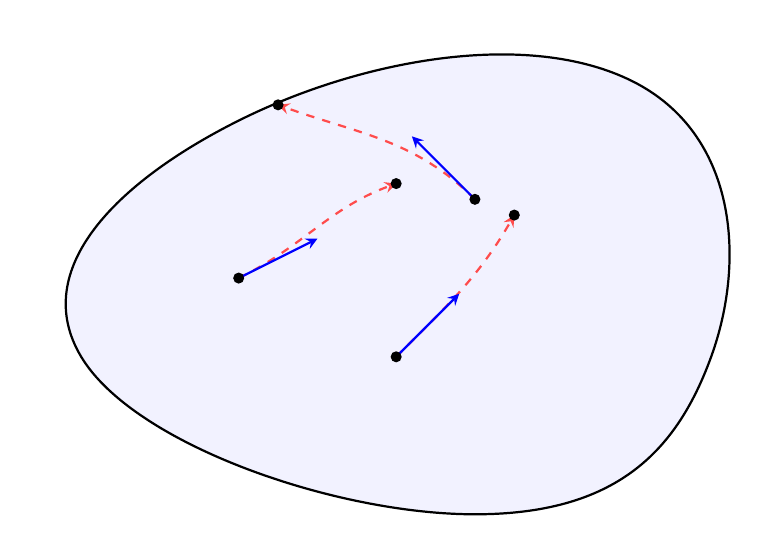
\begin{tikzpicture}[>=stealth]
            % 1. Draw the Manifold
            % Using a smooth cycle to create an organic, topological shape
            \draw[thick, fill=blue!5] plot [smooth cycle, tension=0.8] coordinates {
                    (-2,-1) (0,2) (5,2.5) (6,-1) (3,-3)
                };
            \node[scale=1.5, black!100] at (4.5,-2) {};

            % 2. Define coordinates for the points (q_i)
            \coordinate (q1) at (0,0);
            \coordinate (q2) at (2,-1);
            \coordinate (q3) at (3,1);

            % 3. Define the vectors X(q_i)
            % The vector tips are placed relative to the starting points
            \coordinate (vq1) at (1, 0.5); % Angle ~ 26 degrees
            \coordinate (vq2) at (2.8, -0.2); % Angle = 45 degrees
            \coordinate (vq3) at (2.2, 1.8); % Angle = 135 degrees

            % 4. Define the flowed points \varphi_t(q_i)
            \coordinate (phi1) at (2, 1.2);
            \coordinate (phi2) at (3.5, 0.8);
            \coordinate (phi3) at (0.5, 2.2);

            % 5. Draw the flow lines (Trajectories)
            % The 'out' angle matches the tangent of the vector field at that point
            \draw[->, dashed, thick, red!70] (q1) to[out=26, in=200] (phi1);
            \draw[->, dashed, thick, red!70] (q2) to[out=45, in=240] (phi2);
            \draw[->, dashed, thick, red!70] (q3) to[out=135, in=340] (phi3);

            % 6. Draw the vectors
            \draw[->, thick, blue] (q1) -- (vq1) node[midway, below right] {};
            \draw[->, thick, blue] (q2) -- (vq2) node[midway, below right] {};
            \draw[->, thick, blue] (q3) -- (vq3) node[midway, above right] {};

            % 7. Draw and label the points
            \fill[black] (q1) circle (2pt) node[left] {};
            \fill[black] (q2) circle (2pt) node[left] {};
            \fill[black] (q3) circle (2pt) node[right] {};

            \fill[black] (phi1) circle (2pt) node[right] {};
            \fill[black] (phi2) circle (2pt) node[right] {};
            \fill[black] (phi3) circle (2pt) node[left] {};

        \end{tikzpicture}
    \end{center}
\end{theorem}
\begin{lemma}
    \label{loc:lemaestrela}
    Seja $M$ uma variedade diferenciável, $\varphi:M\to M$ uma aplicação diferenciável, $v \in T_{p}M$ e $f:M\to \mathbb{R}$ diferenciável. Então, $(d\varphi_{p}(v) f)=v(f \circ \varphi(p))$.
    \begin{proof}

        Com efeito, seja $\alpha:(-\epsilon, \epsilon)\to M$ uma curva diferenciável, com $\alpha(0)=p$ e $\alpha'(0)=v$. Temos que
        \begin{align*}
            (d\varphi_{p}(v)f) & =(d\varphi_{p}(\alpha'(0))f)          \\
                               & =(\varphi \circ \alpha)'(0)f          \\
                               & =(f \circ (\varphi \circ \alpha))'(0) \\
                               & =((f \circ \varphi) \circ \alpha)'(0) \\
                               & =\alpha'(0)(f \circ \varphi)          \\
                               & =v(f \circ \varphi)
        \end{align*}
    \end{proof}
\end{lemma}
\begin{lemma}
    \label{loc:5.5_lema_:_possibilidade_de_fatorar_t_de_uma_função}
    Seja $h:(-\delta, \delta)\times U\to \mathbb{R}$ uma aplicação diferenciável, com $h(0, q)=0$, para todo $q \in U$. Existe $g:(-\delta, \delta)\times U\to \mathbb{R}$, com $h(t, q)=tg(t, q)$. Em particular, $g(0, q)=\frac{\partial h(t, q)}{\partial t}|_{t=0}$
    \begin{proof}

        Escrevendo $h(s,q)$, defina
        \begin{equation*}
            g(t,q)=\int_{0}^{1}\frac{\partial h}{\partial s}(ts,q)ds.
        \end{equation*}
        Note que
        \begin{equation*}
            tg(t, q)=\int_{0}^{1}\frac{\partial h}{\partial s}(ts,q)tds
        \end{equation*}
        e que
        \begin{equation*}
            h(t, q)=\int_{0}^{t}\frac{\partial h}{\partial s}(s, q)ds.
        \end{equation*}
        Fazendo $s=tu$, temos que $ds=tdu$, logo, aplicando uma substituição por $u$, segue que
        \begin{equation*}
            h(t,q)=\int_{0}^{1}\frac{\partial h}{\partial s}(tu, q)tdu = tg(t,q).
        \end{equation*}
    \end{proof}
\end{lemma}
\begin{proposition}
    \label{loc:5.4_prop_:_colchetes_como_limite_do_fluxo_local}
    Sejam $X$ e $Y$ campos diferenciaveis de vetores em uma variedade diferenciável $M$. Seja $p \in M$ e $\varphi_{t}$ o fluxo local de $X$ em uma vizinhança $U$ de $p$.
    Então,
    \begin{equation*}
        [X,Y]_{p}=\lim_{ t \to 0 } \frac{1}{t}(Y_{\varphi_{t}(p)}-d\varphi_{t_{p}}Y_{p})
    \end{equation*}
    \begin{proof}

        Seja $f$ uma função real diferenciável em uma vizinhança de $p$.
        Defina $h(t,q):=f(\varphi _{t}(q))-f(q)$. Note que $h(0,q)=0$, logo, pelo lema \Cref{loc:5.5_lema_:_possibilidade_de_fatorar_t_de_uma_função}, existe $g$, tal que $tg(t,q)=f(\varphi_{t}(q))-f(q)$.
        Segue que
        \begin{equation*}
            f \circ \varphi_{t}(q)=tg(t,q)+f(q). \tag{$*$}
        \end{equation*}

        Também pelo lema, temos que
        \begin{align*}
            g(0,q)=\left.\frac{\partial h(t,q)}{\partial t}\right|_{t=0} & =\left.\frac{\partial f \circ\varphi_{t}(q)-f(q)}{\partial t}\right|_{t=0} \\
                                                                         & = \left.\frac{\partial f \circ \varphi(t,q)}{\partial t}\right|_{t=0}      \\
                                                                         & \overset{\text{def}}{=} \frac{\partial \varphi}{\partial t}(0, q)f         \\
                                                                         & =X(\varphi(0, q))f                                                         \\
                                                                         & = X(q)f =X_{q}f=Xf(q) \tag{$**$}
        \end{align*}
        Do \Cref{loc:lemaestrela}, segue que
        \begin{align*}
            (d\varphi_{t_{p}}Y_{p})f & = Y_{p}(f \circ  \varphi_{t})            \\
                                     & \overset{(*)}{=}Y_{p}(tg(t, \cdot)+f)    \\
                                     & =Y_{p}f + Y_{p}(tg(t, \cdot))            \\
                                     & = (Yf)(p)+(tYg(t, \cdot))(p) \tag{$***$}
        \end{align*}

        Também, convém notar que, sendo $g$ uma função diferenciável em uma vizinhança de $p$, temos que
        \begin{align*}
            X_{p}g=X_{\varphi_{0}(p)}g & = X(\varphi_{0}(p))g                                                      \\
                                       & =\frac{\partial \varphi}{\partial t}(0, p)g                               \\
                                       & = \left.\frac{\partial (g \circ  \varphi(t, p))}{\partial t}\right|_{t=0} \\
                                       & =\lim_{ h \to 0 } \frac{g(\varphi(h, p))-g(p)}{h} \tag{$****$}
        \end{align*}

        Segue que
        \begin{align*}
            \lim_{ t \to 0 } \frac{1}{t}(Y_{\varphi_{t}(p)}-d\varphi_{t_{p}}Y_{p})f & = \lim_{ t \to 0 } \frac{1}{t}((Y_{\varphi_{t}(p)})f-(d\varphi_{t_{p}}Y_{p})f)                         \\
                                                                                    & \overset{(***)}{=} \lim_{ t \to 0 } \frac{1}{t}\{(Y_{\varphi_{t}(p)})f-[(Yf)(p)+(tYg(t, \cdot))(p) ]\} \\
                                                                                    & =\lim_{ t \to 0 } \frac{Y_{\varphi_{t}(p)}f - (Yf)(p)}{t} - (Yg(t, \cdot))(p)                          \\
                                                                                    & =\lim_{ t \to 0 } \frac{Yf({\varphi_{t}(p)}) - (Yf)(p)}{t} - (Yg(t, \cdot))(p)                         \\
                                                                                    & \overset{(****)}{=}X_{p}Yf - \lim_{ t \to 0 } (Yg(t, \cdot))(p)                                        \\
                                                                                    & =X_{p}Yf - (Yg(0, \cdot))(p)                                                                           \\
                                                                                    & \overset{(**)}{=}X_{p}Yf - (YXf(\cdot))(p)                                                             \\
                                                                                    & =X_{p}Yf - YXf(p)                                                                                      \\
                                                                                    & = XYf(p) - YXf(p)                                                                                      \\
                                                                                    & = (XYf - YXf)(p)                                                                                       \\
                                                                                    & = (XY-YX)_{p}f                                                                                         \\
                                                                                    & =[X,Y]_{p}f
        \end{align*}

        o que concluí a demonstração.
    \end{proof}
\end{proposition}
Observe que $Y_{\varphi_t(p)}$ indica o valor do campo $Y$ ao longo de uma trajetória do campo $X$, partindo de $p$ após um tempo $t$, enquanto $(d\varphi_t)_p(Y_{p})$ indica o deslocamento infinitesimal ao seguir uma
trajetória do campo $X$ por um tempo $t$, partindo de um ponto a uma distância infinitesimal de
$p$ na direção de $Y_p$.

\textbf{MELHORAR ESSA DESCRIÇÃO AQUI, CREIO NAO ESTAR CLARO, PENSAREI MAIS SOBRE DEPOIS!}
\begin{center}

    \begin{tikzpicture}
        \node[draw, shape=tape, minimum width=84pt, minimum height=71pt, tape bend top=out and in, inner sep=3.93pt, fill=black!36, drop shadow] (node1) at (0.72,2.6) {};
        \node[xscale=0.5, yscale=0.5] at (-0.23,3.22) {$(d\varphi_t)_p(Y_p)$};
        \node[xscale=0.5, yscale=0.5] at (1.02,2.12) {$Y_{p}$};
        \draw[arrows=-Latex] (0.89,2.6) -- (0.8,2.11);


        \draw[fill=black] (0.88,2.6) circle (0.01cm);
        \draw[fill=black] (0.26,2.9) circle (0.01cm);
        \node[xscale=0.5, yscale=0.5] at (0.93,2.72) {$p$};
        \node[xscale=0.5, yscale=0.4] at (2.4,1.36) {$M$};

        \draw[rotate=-7] (0.64,2.76) ellipse [x radius=1.03cm, y radius=0.73cm];
        \node[minimum width=8pt, xscale=0.5, yscale=0.5] at (1.93,3.06) {$U$};


        \draw (0.26,2.91) .. controls (0.27,2.67) and (0.45,2.52) .. (0.62,2.48) .. controls (0.73,2.46) and (0.83,2.49) .. (0.88,2.6);
        \node[xscale=0.5, yscale=0.5] at (0.39,3.04) {$\varphi_{t}\left(p\right)$};
        \node[xscale=0.5, yscale=0.5] at (-0.25,2.52) {$Y_{\varphi_t(p)}$};
        \draw[arrows=-Latex] (0.26,2.91) -- (-0.29,2.66);

        \draw[arrows=-Latex] (0.26,2.9) -- (-0.26,3.11);
    \end{tikzpicture}
\end{center}
Finalizaremos esse capítulo apresentando alguns resultados topológicos acerca das variedades diferenciáveis. Eles serão úteis posteriormente para mostrar que toda variedade diferenciável possui uma métrica.

Retomemos, primeiramente, alguns axiomas topológicos:
\begin{axiom}
    \label{loc:axiomas_sobre_topologia_das_variedades}
    \begin{itemize}
        \item \textbf{Hausdorff:} Dados $p,q \in M$ distintos, existem vizinhanças $U$ e $V$ de $p$ e $q$ respectivamente, tais que $U\cap V=\emptyset$.
        \item \textbf{Base enumerável:} Existe um conjunto enumerável $\mathcal{B}$ de abertos de $M$, tal que todo aberto $U$ de $M$ pode ser escrito como reunião enumerável de elementos de $\mathcal{B}$.
    \end{itemize}
\end{axiom}
\begin{definition}
    \label{loc:def_10_:_familia_localmente_finita_suporte_partição_da_unidade.família_localmente_finita}
    Seja $M$ uma variedade diferenciável e $\{ V_{\alpha} \}$ uma família de abertos de $M$, com $\cup_{\alpha}V_{\alpha}=M$. Tal família é dita localmente finita se para todo $p \in M$ existe $U$ vizinhança de $p$, tal que $U\cap V_{\alpha}\neq \emptyset$ para uma quantidade finita de $\alpha$.
\end{definition}
\begin{definition}
    \label{loc:def_10_:_familia_localmente_finita_suporte_partição_da_unidade.suporte}
    Seja $f:M\to \mathbb{R}$. Dizemos que o suporte de $f$ é o fecho do conjunto $f^{-1}(\mathbb{R}-\{ 0 \})$ e escrevemos $supp(f)$.
\end{definition}
\begin{definition}
    \label{loc:def_10_:_familia_localmente_finita_suporte_partição_da_unidade.partição_da_unidade}
    Seja $\{ f_{\alpha} \}$ uma família de funções reais definidas em $M$. $\{ f_{\alpha} \}$ é dita partição diferenciável da unidade se:
    \begin{enumerate}
        \item Para todo $\alpha$, $f_{\alpha}\geq0$ e $supp(f_{\alpha})\subset V_{\alpha}$, onde $V_{\alpha}=X_{\alpha}(U_{\alpha})$ é uma vizinhança parametrizada;
        \item A família $\{ V_{\alpha} \}$ é localmente finita;
        \item $\sum_{\alpha}f_{\alpha}(p)=1$, para todo $p \in M$.
    \end{enumerate}

    A afirmação 3) tem sentido pois, dado $p \in M$, existe uma vizinhança $U$ de $p$, tal que $U\cap V_{\alpha}\neq \emptyset$ para uma quantidade finita de $\alpha$, isto é, existe um conjunto $A=\{ \alpha_{1}, \dots, \alpha _{k} \}$, tal que $U\cap V_{\alpha}=\emptyset$ se, e somente se, $\alpha \in A$. Logo, se $\alpha \not\in A$, temos que $U\cap V_{\alpha}=\emptyset$, implicando que $p \not\in V_{\alpha}$, isto é, $p \not\in supp(f_{\alpha})$ e, portanto, $f_{\alpha}(p)=0$. Dessa forma, $\sum_{\alpha}f_{\alpha}(p)=\sum_{i=1}^{k}f_{\alpha_{i}}(p)$.
\end{definition}
Além desses, convém mencionar a existência das funções bump, as quais são úteis quando temos algo definido localmente e quisermos estender a definição continuamente.
\begin{lemma}
    \label{loc:def_11_:_funções_bump}
    Considerando o espaço euclidiano $\mathbb{R}^{n}$, dados $p \in \mathbb{R}^{n}$ e uma bola aberta $B(p, r) \subset \mathbb{R}^{n}$, existe uma vizinhança $U$ de $p$, tal que seu fecho $\overline{U} \subset B(p, r)$ e uma função diferenciável $f:\mathbb{R}^{n}\to \mathbb{R}$, tais que $0\leq f(q)\leq1$ para todo $q \in \mathbb{R}$ e
    \begin{equation*}
        f(q)=\left\{\begin{array}{lcl}
            1, & \mbox{se} & q \in \overline{U} \\
            0, & \mbox{se} & q \notin B_{r}(p).
        \end{array}\right.
    \end{equation*}
    Um fato análogo pode ser demonstrado para variedades diferenciáveis.
\end{lemma}
Com isso, exibimos todas as preliminares acerca das variedades diferenciáveis necessárias.